%  LaTeX support: latex@mdpi.com
%  In case you need support, please attach any log files that you could have, and specify the details of your LaTeX setup (which operating system and LaTeX version / tools you are using).

%=================================================================

% LaTeX Class File and Rendering Mode (choose one)
% You will need to save the "mdpi.cls" and "mdpi.bst" files into the same folder as this template file.

%=================================================================

% \documentclass[systems,article,submit,moreauthors,pdftex,12pt,a4paper]{mdpi}
\documentclass[systems,supfile,submit,moreauthors,pdftex,12pt,a4paper]{mdpi}

%--------------------
% Class Options:
%--------------------
% journal
%----------
% Choose between the following MDPI journals:
% actuators, administrativesciences, aerospace, agriculture, agronomy, algorithms, animals, antibiotics, antibodies, antioxidants, appliedsciences, arts, atmosphere, atoms, axioms, batteries, behavioralsciences, bioengineering, biology, biomedicines, biomimetics, biomolecules, biosensors, brainsciences, buildings, cancers, catalysts, cells, challenges, chemosensors, children, chromatography, climate, coatings, computation, computers, cosmetics, crystals, data, dentistryjournal, diagnostics, diseases, diversity, econometrics, economies, education, electronics, energies, entropy, environmentalsciences, environments, epigenomes, fibers, foods, forests, futureinternet, galaxies, games, gels, genealogy, genes, geosciences, healthcare, horticulturae, humanities, hydrology, informatics, information, inorganics, insects, ijerph, ijfs, ijms, ijgi, jcdd, jcm, jdb, jfb, jimaging, jof, joi, jlpea, jmse, jpm, jrfm, jsan, land, laws, life, lubricants, machines, marinedrugs, materials, mathematics, medicalsciences, membranes, metabolites, metals, microarrays, micromachines, microorganisms, minerals, molbank, molecules, nanomaterials, ncrna, nutrients, pathogens, pharmaceuticals, pharmaceutics, pharmacy, photonics, plants, polymers, processes, proteomes, publications, religions, remotesensing, resources, risks, robotics, safety, sensors, sinusitis, socialsciences, societies, sports, standards, sustainability, symmetry, systems, technologies, toxics, toxins, universe, vaccines, veterinarysciences, viruses, water
%---------
% article
%---------
% The default type of manuscript is article, but could be replaced by using one of the class options:
% article, review, communication, commentary, bookreview, correction, addendum, editorial, changes, supfile, casereport, comment, conceptpaper, conferencereport, meetingreport, discussion, essay, letter, newbookreceived, opinion, projectreport, reply, retraction, shortnote, technicalnote, creative, datadescriptor (for journal Data)
%----------
% submit
%----------
% The class option "submit" will be changed to "accept" by the Editorial Office when the paper is accepted. This will only make changes to the frontpage (e.g. the logo of the journal will get visible), the headings, and the copyright information. Journal info and pagination for accepted papers will also be assigned by the Editorial Office.
% Please insert a blank line is before and after all equation and eqnarray environments to ensure proper line numbering when option submit is chosen
%------------------
% moreauthors
%------------------
% If there is only one author the class option oneauthor should be used. Otherwise use the class option moreauthors.
%---------
% pdftex
%---------
% The option "pdftex" is for use with pdfLaTeX only. If eps figure are used, use the optioin "dvipdfm", with LaTeX and dvi2pdf only.

%=================================================================
\setcounter{page}{1}
\lastpage{x}
\doinum{10.3390/------}
\pubvolume{xx}
\pubyear{2015}
%\externaleditor{Academic Editor: xx}
\history{Received: xx / Accepted: xx / Published: xx}
%------------------------------------------------------------------
% The following line should be uncommented if the LaTeX file is uploaded to arXiv.org
%\pdfoutput=1

%=================================================================

% Add packages and commands to include here
% The amsmath, amsthm, amssymb, hyperref, caption, float and color packages are loaded by the MDPI class.
%\usepackage{graphicx}
%\usepackage{subfigure,psfig}
%%% 한글 사용 
\usepackage{kotex}
% \usepackage[unicode]{hyperref}

\usepackage{dhucs-cmap}  % 한글 깨짐 방지

\usepackage{graphicx}
%\usepackage{caption}
\usepackage{subcaption} 
\usepackage{stfloats}

\usepackage{comment}  % comment 태그

\usepackage{multirow}

\newcommand{\JHMEMO}[1]{\textcolor{red}{#1}}


% create a shortcut to typeset table headings
\newcommand\tabhead[1]{\small\textbf{#1}}

%=================================================================
%% Please use the following mathematics environments:
% \theoremstyle{mdpi}
% \newcounter{thm}
% \setcounter{thm}{0}
% \newcounter{ex}
% \setcounter{ex}{0}
% \newcounter{re}
% \setcounter{re}{0}
%
% \newtheorem{Theorem}[thm]{Theorem}
% \newtheorem{Lemma}[thm]{Lemma}
% \newtheorem{Corollary}[thm]{Corollary}
% \newtheorem{Proposition}[thm]{Proposition}
%
% \theoremstyle{mdpidefinition}
% \newtheorem{Characterization}[thm]{Characterization}
% \newtheorem{Property}[thm]{Property}
% \newtheorem{Problem}[thm]{Problem}
% \newtheorem{Example}[ex]{Example}
% \newtheorem{ExamplesandDefinitions}[ex]{Examples and Definitions}
% \newtheorem{Remark}[re]{Remark}
% \newtheorem{Definition}[thm]{Definition}
%% For proofs, please use the proof environment (the amsthm package is loaded by the MDPI class).

%=================================================================

% Full title of the paper (Capitalized)
\Title{Using Portable Multiscreen Interactive Surface for Construction Information Visualization}

% Authors (Add full first names)
\Author{Jonghoon Seo $^{1,\dagger}$, Seungho Chae $^{1,\dagger}$, Yoonsik Yang $^{1,\dagger}$ and Tack-Don Han $^{1,}$*}

% Affiliations / Addresses (Add [1] after \address if there is only one affiliation.)
\address[1]{
$^{1}$ Institute 1, University 1, Full Address, City, Country}

\contributed{$^\dagger$ These authors contributed equally to this work.}

% Contact information of the corresponding author (Add [2] after \corres if there are more than one corresponding author.)
\corres{e-mail, telephone and fax number of the corresponding author.}

% Abstract (Do not use inserted blank lines, i.e. \\)
\abstract{This is the abstract section. The abstract should be one section and count less than 200 words.}
% %!TEX root = ../Sensors_SmartConstruction.tex
% -*- root: ../Sensors_SmartConstruction.tex -*-

%--------------------------------------------------------------------------
%	Abstract
%	목표 분량: 150 단어 정도

\begin{abstract}

% 한글 버전
건축 공정은 다양한 Stakeholder들이 참여하여 서로 협업을 수행하여 달성된다. 하지만 현재의 건축 현장은 설계자(architect)의 건축 도면이 시공 현장에서 충분히 접근되고 검토되지 않는 문제가 있다. /textit{또한 현장에서의 수정사항이 전체 모델에 일관적으로 반영되기 어렵고, 작업자 사이에서 이러한 변경 정보가 공유되기 어렵다는 문제가 있다.} 이는 현장에서(on-site) 사용하기에는 시스템 구성이 너무 복잡하거나 3차원 모델의 정보가 제공되지 않고, 입력기술이 복잡하여 현장에서의 작업 내역을 반영하기 어렵기 때문이다. 본 논문에서는 이러한 문제점을 해결하기 위하여 포터블 Projection AR 기술을 이용하여 2D와 3D Dual Workspace를 제공하고, IT 기술에 익숙하지 않은 건설-근로자(construction worker)들이 직관적으로 시스템을 사용하도록 하기 위하여 펜과 손가락의 2D/3D Bimanual Interaction를 설계하였다. \textit{또한 모바일 컴퓨팅 기술을 이용하여 작업 중에도 편리하게 전체 건축 모델의 정보를 이용하고 수정사항을 빠르게 모델에 반영하며, 이를 통하여 쉽게 커뮤니케이션이 가능하도록 하였다. 그리고 이러한 시스템을 이용한 Interaction을 Design하였다. 이러한 시스템과 상호작용 설계를 이용하여 건축 관련자들에게 사용하도록 하고 기존의 도면 기반의 방법과 과업(task) 수행 시간을 비교하고 제안하는 시스템의 informal user study를 수행하여 현장에서 유용성이 높음을 확인하였다.}


% 영어 버전
% %!TEX root = ../sigchi-sample.tex

\begin{comment}
In the construction process, various stakeholders attend and cooperate with each other to move the project forward. However, it is currently difficult for architects' blueprints to be sufficiently adapted on a construction site, and there are many problems that have not been considered. It is also difficult to reflect modifications made on-site in overall models, and the difficulty in sharing this changed information between workers can be a problem. This system construction may be too complicated to be used on-site or 3D model information may not be offered, and since input technology is complicated, it is difficult to reflect this work information on-site. This study offers a 2D and 3D Dual Workspace using portable Projection AR to solve these problems, and 2D/3D Bimanual Interaction for pen and fingers was designed so that construction workers unused to IT can intuitively use the system. The system makes convenient use of overall construction model information using mobile computing technology within construction work, and modifications are quickly reflected in its model. Through this, it allows for easy communication. This system was designed to use interaction. It is designed for use by construction managers using an interactive design. Informal user studies were carried out for the proposed system comparing previous blueprint-based methods and task operation time to verify increased on-site usability. 
\end{comment}

% Editage 버전
Various stakeholders participate in construction and cooperate to move a project forward. However, it is difficult to adapt blueprints adequately on a construction site or to reflect modifications made on site in overall models, and sharing this changed information among workers. This study offers a 2D and 3D dual workspace using portable projection augmented reality to solve these problems and 2D/3D bimanual interaction for pen and fingers designed to enable construction workers unaccustomed to information technology to use the system intuitively. The system uses overall construction model information with mobile computing technology in construction work, with modifications being quickly reflected in its model, allowing for easy communication. This system was designed to be used by construction managers using an interactive design. Informal user studies were conducted for the proposed system comparing previous blueprint-based methods and task operation time to verify increased on-site usability.


%%%%%%%%%%%%%%%%%%%%%%%%%%%% UbiComp 버전
% 제임스 버전
\begin{comment}
Collaboration among stakeholders in the construction process is vital to completing projects successfully and on time. However, contruction engineers face the challenging problem of looking  at various architectural drawing perspectives. The perspectives can be complex, specific to a specialized job, and does not show a complete 3D view of the building. In this paper, we solve this problem by using Portable Projection AR technology to provide 2D and 3D dual workspace giving both a familar workspace feel and an intuitive system using pen and fingers for 2D/3D bimanual interaction. Based on feedback responses from construction workers who evaluated our prototype our system is shown to be more convenient and intuitive accessing information from construction drawings.
\end{comment}


% 번역소 버전
\begin{comment}
Construction processes are achieved by executing cooperation each other from diverse stakeholders' participation. But, at present construction sites, there is a problem that construction blueprints of architects are not approached and examined enough. This is because the system configuration is too complicated, 3D model information is not provided, or on-site work records are not reflected on the blueprints. To solve these problems, this paper provides 2D and 3D dual workspaces using projection AR technology. Also, in order that construction workers unfamiliar with IT technology can use systems intuitively, 2D/3D bimanual interaction of pens and fingers was designed. Through them, targeting real construction workers, from evaluating video prototypes, it was confirmed to access to construction blueprints and information more conveniently and intuitively on site.
\end{comment}
%%%%%%%%%%%%%%%%%%%%%%%%%%%% UbiComp 버전

\end{abstract}

%--------------------------------------------------------------------------
%	Keywoards
\keywords{
Interactive 3D surface; smart space; bimanual interaction; smart construction
}

\category{H.5.2.}{Information Interfaces and Presentation (e.g. HCI)}{User Interfaces}


% Keywords: add 3 to 10 keywords
\keyword{keyword; keyword; keyword}

% The fields PACS, MSC, and JEL may be left empty or commented out if not applicable
%\PACS{}
%\MSC{}
%\JEL{}

% If this is an expanded version of a conference paper, please cite it here: enter the full citation of your conference paper, and add $^\dagger$ in the end of the title of this article.
%\conference{}

%%%%%%%%%%%%%%%%%%%%%%%%%%%%%%%%%%%%%%%%%%
% For journal Data:

%\dataset{DOI number or link to the deposited data set in cases where the data set is published or set to be published separately. If the data set is submitted and will be published as a supplement to this paper in the journal Data, this field will be filled by the editors of the journal. In this case, please make sure to submit the data set as a supplement when entering your manuscript into our manuscript editorial system.}
%\datasetlicense{license under which the data set is made available (CC0, CC-BY, CC-BY-SA, CC-BY-NC, etc.)}

%%%%%%%%%%%%%%%%%%%%%%%%%%%%%%%%%%%%%%%%%%

\begin{document}

%%%%%%%%%%%%%%%%%%%%%%%%%%%%%%%%%%%%%%%%%%

%!TEX root = ../Sensors_SmartConstruction.tex
% -*- root: ../Sensors_SmartConstruction.tex -*-

\section{Introduction}

% 한글버전
%%!TEX root = ../construction.tex
% -*- root: ../construction.tex -*-

% 유비쿼터스 기술과 HCI 기술의 발전으로 다양한 산업 분야에서 좀 더 편리하고 seamless하게 컴퓨터를 활용하고 있다. 특히 현대 건축 분야는 새로운 컴퓨팅 기술을 이용하여 architect의 창의성을 높이고 다양한 stakeholder 들 간의 커뮤니케이션을 보조하기 위한 다양한 연구들이 이루어지고 있다. 하지만 여전히 건축 현장의 작업자들은 이러한 새로운 기술을 비롯하여 컴퓨터 인터페이스에 익숙하지 못하며, old-fashion 으로 작업을 진행하고 있다. 이에 따라 설계자(architect)의 의도가 실제 건축물에 충분히 반영되지 못하며, 이러한 과정에서 경제적, 안전적, 설계적 문제점들이 발생할 가능성이 있다. 따라서 이러한 문제점들을 해결하기 위하여 건축 현장에서(on-site) 향상된 IT 기술을 이용하여 실시간으로 건축 정보를 획득하고 이용하기 위한 연구들이 진행되고 있다.\textit{ 이러한 기술들은 현장(on-site)에서 적용이 가능하도록 포터블하거나 웨어러블 형태로 설계되어야 하며\cite{song_penlight:_2009, yeh_-site_2012}, 현실 세계의 3차원 공간에 쉽게 매핑할 수 있도록 3차원 데이터를 직관적으로 제공하여야 한다\cite{chi_research_2013, kim_interactive_2012, yeh_-site_2012}. 또한, 현장에서 발생되는 수정사항이나 업데이트 정보를 실시간으로 전체 모델에 반영하도록 수정사항을 입력하기 위한 인터페이스도 필요하며\cite{song_penlight:_2009}, 이러한 입력 정보를 통합하여 전체 모델의 정보가 consistent하게 유지하도록 하는 integrated BIM 기술도 중요하다. }

% 본 논문은 이러한 문제점을 극복하고 건축 현장에서 실제로 활용이 가능한 시스템을 제공하기 위하여 Interactive 3D Smart Space 기술\cite{grossman__2010}과 Mobile Computing 기술을 활용하였다. 특히, Interactive 3D Smart Space 기술의 문제점인 Portablity 문제를 해결하기 위하여 모바일 프로젝터와 깊이 인식 카메라를 사용하였다. 이를 이용하여 건축물의 'L'-shape 벽면에 걸쳐 프로젝션함으로써 2D Interaction 을 위한 Horizontal Screen과 3D Interaction을 위한 Vertical Screen을 구성하였다. 이러한 환경에서 NUI 기술을 이용하여 직관적으로 3차원 정보를 획득하고 상호작용 하도록 하였다. \textit{ 또한, 모바일 폰을 이용하여 작업 중에도 건축 정보에 접근할 수 있도록 하였다. 이러한 시스템을 이용하여, Shared workspace로써의 Interactive 3D Smart Space의 정보와 Personal workspace로써의 모바일 폰의 정보 간의 seamless한 정보의 공유 및 integration을 제공한다. 이를 통하여 건설 현장에서도 seamless하게 건축 정보를 접근하면서 실시간으로 건축 모델의 정보를 업데이트하고, 작업 중에도 편리하게 협업할 수 있는 시스템을 설계하였다. } 본 논문에서는 이러한 시스템을 이용하여 건축 현장에 적용하기 위한 design을 수행하고, /textit{이를 건축 관련자들에게 사용 후 informal user study와 비교 연구를 적용하여 시스템의 유용성을 검증하였다.} 추가적으로 실험의 피드백과 구현 상의 문제들을 정리하고 결론을 도출하였다.

%% 이 밑에 내용이 있었음
% 현대 건축 분야는 새로운 컴퓨팅 기술을 이용하여 architect의 창의성을 높이고 다양한 stakeholder 들 간의 커뮤니케이션을 지원하기 위한 다양한 연구들이 이루어지고 있다. 하지만 여전히 건축 현장의 작업자들은 여러 현실적인 문제로 old-fashion 으로 작업을 진행하고 있다\cite{behzadan_visualization_2005}. 이에 따라 설계자(architect)의 의도가 실제 건축물에 충분히 반영되지 못하며, 이러한 과정에서 경제적, 안전적, 설계적 문제점들이 발생할 가능성이 있다. 따라서 이러한 문제점들을 해결하기 위하여 건축 현장에서(on-site) 향상된 IT 기술을 이용하여 실시간으로 건축 정보를 획득하고 이용하기 위한 연구들이 진행되고 있다. 이러한 기술들은 현장(on-site)에서 적용이 가능하도록 포터블하거나 웨어러블 형태로 설계되어야 하며\cite{song_penlight:_2009, yeh_-site_2012}, 현실 세계의 3차원 공간에 쉽게 매핑할 수 있도록 3차원 데이터를 직관적으로 제공하여야 한다\cite{chi_research_2013, kim_interactive_2012, yeh_-site_2012}. 또한, 현장에서 발생되는 수정사항이나 업데이트 정보를 실시간으로 전체 모델에 반영하도록 수정사항을 입력하기 위한 인터페이스도 필요하며\cite{song_penlight:_2009}, 이러한 입력 정보를 통합하여 전체 모델의 정보가 consistent하게 유지하도록 하는 integrated BIM 기술도 중요하다.

% 본 논문은 이러한 문제점을 극복하고 건축 현장에서 실제로 활용이 가능한 시스템을 제공하기 위하여 3D Interactive Surface 기술\cite{grossman__2010}과 Mobile Computing 기술을 활용하였다. 특히, 3D Interactive Surface 기술의 문제점인 Portablity 문제를 해결하기 위하여 모바일 프로젝터와 깊이 인식 카메라를 사용하였다. 이를 이용하여 작업 환경의 'L'-shape 벽면에 걸쳐 프로젝션함으로써 2D Interaction 을 위한 Horizontal Screen과 3D Interaction을 위한 Vertical Screen을 구성하였다. 이러한 환경에서 NUI 기술을 이용하여 직관적으로 3차원 정보를 조작하고 상호작용 하도록 하였으며, Anoto Pen 기술로 도면 정보를 실시간으로 반영하도록 하였다. 또한, 모바일 폰을 이용하여 작업 중에도 건축 정보에 접근할 수 있도록 하였다. 이러한 시스템을 이용하여, Shared workspace로써의 3D Interactive Surface의 정보와 Personal workspace로써의 모바일 폰의 정보 간의 seamless한 정보의 공유 및 integration을 제공한다. 이를 통하여 건설 현장에서도 seamless하게 건축 정보를 접근하면서 실시간으로 건축 모델의 정보를 업데이트하고, 작업 중에도 편리하게 협업할 수 있는 시스템을 설계하였다. 본 논문에서는 이러한 시스템을 이용하여 건축 현장에 적용하기 위한 design을 수행하고, 이를 건축 관련자들에게 사용 후 informal user study와 비교 연구를 적용하여 시스템의 유용성을 검증하였다. 추가적으로 실험의 피드백과 구현 상의 문제들을 정리하고 결론을 도출하였다.

현재 건축 시공 현장에서의 문제점 
\begin{itemize} 
\item 건축 관계자들, 특히 설계자와 시공자 사이의 Communication 문제
\item 도면 활용도 저하 
\end{itemize}

% 영어버전
% %!TEX root = ../sigchi-sample.tex

\begin{comment}
Today's industries are using the power of ubiquitous technologies and human computer interaction (HCI) technology to make work as seamless as possible. Especially in the field of modern architecture, architects are using new computing technology to enhance creativity and aid in communication between various stakeholders. Still, construction engineers on-site may not be familiar with new technology and instead use old-fashion tools to understand the architect's drawings. As a result, management and communication of the architect's design plan may not be followed according to his or her overall specifications which can cause increase in budget costs, confusion in safety factors, and poor building design.
A number of studies using enhanced IT technologies have been developed to help manage and communicate the task of acquiring real-time information that may not otherwise be available on hand. These technologies must be designed to be portable or wearable so they can be used on-site\cite{song_penlight:_2009, yeh_-site_2012}, and must offer intuitive use of 3D data so they can easily map 3D spaces in the real world \cite{chi_research_2013, kim_interactive_2012, yeh_-site_2012}. They also need interfaces for input of modifications in order to reflect adjusted or updated information occurring on-site in the overall model in real-time\cite{song_penlight:_2009}, and integrated BIM technology is important to combine entered information and keep the overall model's information consistent. 
In this paper, we applied \textit{interactive 3D Smart Sapce}\cite{grossman__2010} and \textit{Mobile Computing} to solve the portability problem and providing a feasible interface for on-site construction work. To make our system portable, we used a small depth camera and portable projector to recognize the geometry of the world and to project additional information. Using an 'L'-shape wall presents at work sites, our system projects content onto a vertical wall and horizontal surface allowing 2D interaction to take place on the horizontal surface and 3D interaction on the wall. This natural user interface (NUI) makes for an intuitive aid in construction work providing additional 3D information to interact with. 


In addition, we incorporate the use of an Anato Pen to allow the user to make modifications in real-time while on the job site. We conducted an informal study with participants who are involved in the construction process to evaluate our system. The remainder of this paper examines the feedback from the participants, implementation and experiment results of the drawing functions. Furthermore, construction information can be seen on the work site using a mobile phone. Using this system, seamless information sharing and integration are offered between mobile phones through a shared workspace, Interactive 3D Smart Space and personal workspace. Through this, construction information can be used seamlessly on the construction site as well while the construction model information is updated in real-time with this system designed to enable convenient on-the-job cooperation. The system in this paper is designed for application on construction sites, and after use, informal user studies were conducted on construction managers to verify the usefulness of this system through comparative research. Additionally, experiment feedback and difficulties in realizing the experiment were considered to infer a conclusion.
\end{comment}

Today's industries use ubiquitous computing and human computer interaction technologies to make work as seamless as possible. Especially in modern architecture, architects are using new computing technology to enhance creativity and aid in communication between various stakeholders. Nevertheless, construction engineers on site might not be familiar with new technology, using old-fashioned tools to understand an architect's drawings. As a result, management and communication of an architect's design plan might not be conducted according to his or her overall specifications, potentially causing increased budget costs, confusion in safety factors, and poor building design. A number of studies using enhanced information technologies have been developed to help manage and communicate the acquisition of real-time information that might not be available otherwise. These technologies must be designed to be portable or wearable to enable them to be used on site \cite{song_penlight:_2009, yeh_-site_2012} and must offer intuitive use of 3D data to enable easy mapping of 3D spaces in the real world \cite{chi_research_2013, yeh_-site_2012}. They also need interfaces for input of modifications to reflect information adjusted or updated on site in the overall model in real-time \cite{song_penlight:_2009}, and integrated building information modeling (BIM) technology is important to combine entered information and keep the overall model's information consistent. 

\begin{figure}[b!]
\centering
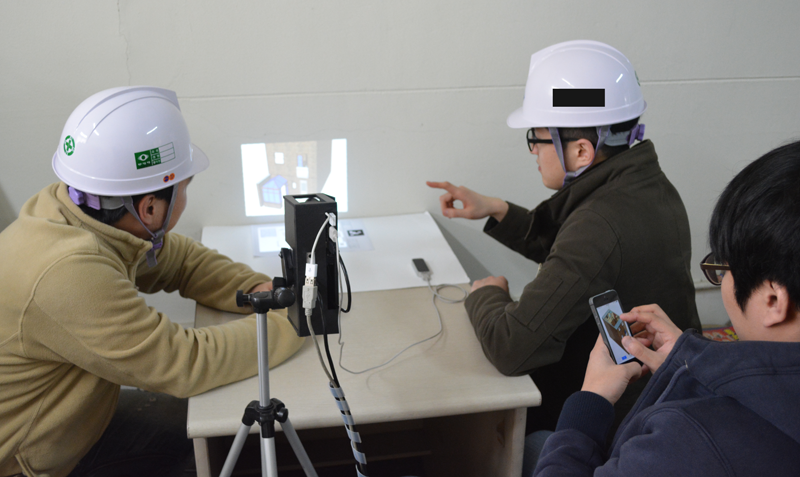
\includegraphics[width=1.0\columnwidth, height=5cm]{1-Introduction/proposed_system}
\caption{Prototype of Port3DAr}
\label{fig:prototype}
\end{figure}
\modified{In this paper, we combine interactive 3D smart spaces \cite{grossman__2010} and mobile computing to solve the portability problem and provide a feasible interface for on-site construction work. To make our system portable, we used a portable depth camera and projector to recognize the geometry of the world and to project additional information. Using an L-shaped wall present at work sites, our system projects content onto a vertical wall and horizontal surface, allowing 2D interaction to take place on the horizontal surface and 3D interaction on the wall. This natural user interface (NUI) provides an intuitive aid in construction work and additional 3D information to interact with. In addition, we incorporate the use of an Anoto Pen to allow the user to make modifications in real-time while on the job site.}


\modified{ Furthermore, construction information can be seen on the work site using a mobile devices. With this system in use, seamless information sharing and integration are offered between mobile devices through a shared workspace, interactive 3D smart space, and personal workspace. As a result, construction information can be used seamlessly on the construction site, while the construction model information is updated in real time, with the system being designed to enable convenient on the job cooperation. The proposed system is designed for use on construction sites, and informal user studies were conducted of construction managers after use to verify the usefulness of this system through comparative research. Additionally, experiment feedback and difficulties in conducting the experiment were considered to draw conclusions.}

% 재작성 한글 버전
%!TEX root = ../Sensors_SmartConstruction.tex
% -*- root: ../Sensors_SmartConstruction.tex -*-

건축 산업(Construction Industry)에 IT 기술을 적용하여 기존 건축 산업의 문제를 극복하고자 하는 연구들이 다양하게 진행되고 있다. 이러한 연구들이 해결하고자 하는 문제는, 첫번째로 건축 작업에서 원하는 정보를 적절하게 제공해줌으로써 정확한 건축물을 지을 수 있도록 하는 것이다. 이를 위해서는 실제 현장에서 획득하기 힘든 정보를 즉각적으로 제공하여야 하고\cite{yeh_-site_2012,cote_augmented_2013,chi_research_2013}, 2D 데이터 뿐만이 아니라 다양한 형태의 정보를 제공함으로써 현장 근로자가 적절한 정보를 제공받을 수 있도록 하여야 한다\cite{behzadan_ubiquitous_2008,schall_handheld_2009}. 

다음으로 해결하고자 하는 문제는, 건축 작업에 참여하는 다양한 관련자들(stakeholder) 사이의 효율적인 의사소통을 지원하고자 하는 것이다. 건축 작업에는 다양한 전문가가 참여하고, 다양한 문제들이 발생한다. 따라서, 효율적인 의사소통이 지원되지 않을 경우에 작업의 비용과 기간이 증가할 뿐만 아니라\cite{schall_handheld_2009}, 건축물의 안전성도 떨어지게 된다\cite{wagner_building_2012,lin_using_2014}. 따라서 IT 기술을 활용하여 관련자들 사이의 커뮤니케이션을 지원하여 빠르고 정확하게 의사결정을 이루는 것이 중요하다. % 본 논문에서는 이러한 문제점들을 해결하기 위하여 2D 데이터에서부터 건축물의 전체적인 3차원 모형, 내부 벽면에 숨겨진 정보까지 다양한 건축물의 정보를 동시에 제공하고 이를 수정할 수 있도록 하는 포터블 기기를 제안한다. 또한, 건축 현장에서의 커뮤니케이션을 지원하기 위하여 프로젝션 기술을 이용하여 구현함으로써 서로 다른 전문가들이 현장에서 참여하여 의사소통할 수 있도록 하였다.


% 첫번째 문제를 해결하기 위하여, 건축 현장에서 필요한 정보를 적절하게 제공하기 위한 다양한 연구가 이루어지고 있다. 이러한 연구는 제공되는 정보의 종류에 따라 2D data, 3D model, MEP(Mechanical, Electronical, and Plumbing) 기반의 연구로 구분할 수 있다\cite{ebbesen_information_2015}. 
이러한 문제점을 극복하기 위하여 건축현장에서 IT기술을 활용하는 다양한 연구들이 이루어지고 있다. 이 연구들은 제공되는 정보의 종류에 따라 2D Data, 3D Model, MEP 기반의 연구로 분류된다. 2D Data 정보의 경우, 도면 정보를 기반으로 상세한 건축 정보를 제공받을 수 있지만\cite{yeh_-site_2012,ishii_augmented_2002,cote_augmented_2013}, 3차원 모델 정보의 제공이 부족하므로 이를 해석하는 과정에서 Image Mismatch가 발생하기 쉽다. 이러한 문제점을 극복하기 위해 2D Data를 이용하여 3D 모델을 제공하는 연구들이 제시되었다\cite{wagner_building_2012,dong_collaborative_2013, hou_combining_2014,behzadan_ubiquitous_2008,williams_bim2mar:_2015}. 이러한 연구는 현실 환경과 같이 최종 건축물의 3차원 정보를 조망할 수 있다는 장점이 있으나, 건축 현장의 세부적인 정보를 획득하기에 어려움이 존재한다. 

최근에는 이러한 정보를 제공하기 위하여 Building Information Management(BIM) 정보를 기반으로 건축물 내의 감춰진 Mechanical, Electronic, and Plumbing (MEP) 구조물의 정보를 제공하는 연구가 진행되고 있다\cite{schall_handheld_2009,olbrich_augmented_2013,kwon_defect_2014,webster_augmented_????,golparvar-fard_d4ar4-dimensional_2009}. 이러한 연구는 건축물 부분의 세부 정보를 획득할 수 있으나, 전체적인 구조를 파악하기 어려웠다\cite{webster_augmented_????}. 본 논문에서는 효율적인 정보 제공을 위해 2D 데이터에서부터 건축물의 전체적인 3D 모델과 내부 벽면에 숨겨진 MEP 정보까지 전체적인 정보를 제공하고자 하였다. 특히, 이러한 다양한 정보를 종합적으로 제공하기 위하여 Multi-view 기반의 Interactive Screen 기술을 이용하여 이러한 정보들을 효율적으로 제공하는 시스템을 제안하였다

% 두번째 문제를 해결하기 위하여, IT 기술을 이용하여 다양한 관계자 사이의 효율적인 의사소통을 제공하기 위한 다양한 연구가 진행되고 있다\cite{ishii_augmented_2002,klein_imaged-based_2012,chi_development_2012,lin_using_2014}. 
이러한 연구들은 커뮤니케이션 환경에 따라 Desktop 환경에서 모바일 기기 환경, Projection 기반의 Interactive Surface 환경으로 진화하였다. 먼저, Desktop 기반의 연구\cite{dong_collaborative_2013,golparvar-fard_d4ar4-dimensional_2009,lin_using_2014}들은 고정적인 환경인 Off-Site에서 진행되며, 전체적인 조망이나 정보 공유가 가능하다. 이러한 연구들의 경우, Off-Site에서의 협업은 가능하나 시스템 구조상 On-Site 에서는 활용되기 어렵다는 단점이 있다. 이러한 단점을 극복하기 위해 On-Site에서 동작 가능한 모바일 기반의 연구들\cite{saidi_value_????,kwon_defect_2014,cote_augmented_2013,irizarry_ambient_2014,hammad_distributed_2009,bae_high-precision_2013,ammari_collaborative_2014,williams_bim2mar:_2015}이 진행되었다. 실제 건축 현장에서 Mobile Augmented Reality 기술을 이용하여 도면이나 3D 모델 등의 정보를 확인 할 수 있고, 필요에 따라 수정 가능하다. 하지만 모바일 기기의 특성상 화면 공유보다는 개인을 위한 Personal Workspace를 제공하기 때문에 협업에 제한적이다. 

이러한 문제를 극복하기 위해, Desktop과 Mobile 기반 연구들의 단점을 보완하여 On-Site 에서 건축 관계자들의 협업을 지원하기 위해 Projection 기반의 Interactive surface 기반의 연구들\cite{ishii_augmented_2002,wagner_building_2012,song_penlight:_2009}이 제시되고 있다. 이러한 기술은 Projection 기술을 이용하여 Interaction Space를 제공하기 때문에 여러 사용자들이 참여하여 협업하기에 적합하다. 따라서, 현장에서의 효율적인 의사소통을 위해서는, 개인화 된 기기 보다는 여러 사용자의 참여가 가능한 Projection 기반의 Interactive Surface 기술을 이용하는 것이 적합하다.




%이러한 문제를 극복하기 위하여 건축 관계자들 간의 협업을 위해 다양한 연구들이 진행되고 있다. 먼저, Desktop 기반의 연구[3, 15, 21]들은 고정적인 환경인 Off-Site에서 진행되며, 전체적인 조망이나 정보 공유가 가능하다. 이러한 연구들의 경우, Off-Site 에서의 협업은 가능하나 시스템 구조상 On-Site에서는 활용되기 어렵다는 단점이 있다. 이러한 단점을 극복하기 위해 On-Site에서 동작 가능한 모바일 기반의 연구들[2, 11, 12, 17-19]이 진행되었다. 실제 건축 현장에서 Mobile Augmented Reality 기술을 이용하여 도면이나 3D 모델 등의 정보를 확인 할 수 있고, 필요에 따라 수정 가능하다. 하지만 모바일 기기의 특성상 화면 공유보다는 개인을 위한 Personal Workspace를 제공하기 때문에 협업에 제한적이다. 이러한 문제를 극복하기 위해, Desktop과  Mobile 기반 연구들의 단점을 보완하여 On-Site에서 건축 관계자들의 협업을 지원하기 위해 Projection 기반의 Interactive surface 기반의 연구들[4, 8, 10, 20]이 제시되고 있다. 이러한 기술은 Projection 기술을 이용하여 Interaction Space를 제공하기 때문에 여러 사용자들이 참여하여 협업하기에 적합하다. 따라서, 현장에서의 효율적인 의사소통을 위해서는, 개인화 된 기기 보다는 여러 사용자의 참여가 가능한 Projection 기반의 Interactive Surface 기술을 이용하는 것이 적합하다.

% 또한, 시스템적으로 가상현실 기술 기반, 모바일 어플리케이션 기반, 증강현실 기술 기반, Interactive Surface 기반의 연구들이 진행되고 있다. 가상현실 기술 기반의 연구들\cite{lin_using_2014,dong_collaborative_2013}들은 현장보다는 사전 준비 단계에서 활용되며, 전체적인 조망이 가능하다는 장점이 있으나, 시스템 구조 상 on-site에서는 활용되기 어렵다는 문제가 있다. xxx

%%%%%%


% 본 논문은 이러한 문제점을 극복하고 건축 현장에서 실제로 활용이 가능한 시스템을 제공하기 위하여 Interactive Surface 기술\cite{grossman__2010} 기반의 2D/3D 건축 정보 Visualization System을 제안한다. 특히, 건축 현장에서 활용도를 높이기 위하여 모바일 프로젝터와 깊이 인식 카메라를 이용하여 portable 시스템을 구현하였다. 기존 Interactive Surface 기술과 다르게 2D/3D 정보를 동시에 보여주기 위하여 Multiscreen Interactive Surface 기술을 적용하였으며, Portable 하게 Multiscreen을 구현하기 위하여 Image Marker 기반의 Calibration 기술을 개발하여 미리 설치된 환경이 아니라 실시간으로 Multiscreen을 구성하도록 하였다. 이를 이용하여 현장의 'L'-shape 벽면에 걸쳐 프로젝션함으로써 2D Interaction 을 위한 Horizontal Screen과 3D Interaction을 위한 Vertical Screen을 구성하였다. 이를 통하여 건설 현장에서도 쉽고 빠르게 건축 정보에 접근함으로써 현장에서의 협업을 높일 수 있었다. 

% 하면서 실시간으로 건축 모델의 정보를 업데이트하고, 작업 중에도 편리하게 협업할 수 있는 시스템을 설계하였다. 본 논문에서는 이러한 시스템을 이용하여 건축 현장에 적용하기 위한 design을 수행하고, 이를 건축 관련자들에게 사용 후 informal user study와 비교 연구를 적용하여 시스템의 유용성을 검증하였다. 추가적으로 실험의 피드백과 구현 상의 문제들을 정리하고 결론을 도출하였다.
% 논문의 구성은 2장에서 제안하는 시스템의 구조와 HW, SW 설계 및 구현, 상호작용 설계에 대하여 설명한다. 3장에서는 사용자 대상의 실험 설계 및 결과에 대하여 서술하고, 4장에서 실험 결과에 대한 discussion을 기술한다. 그리고 5장에서 결론을 짓도록 한다.

본 논문에서는 건축 작업 시 현장에서 필요한 2차원 건축 정보부터 3차원 모델 뷰와 숨겨진 MEP 정보까지, 다양한 정보가 동시에 필요한 문제를 해결하고, 이를 통하여 현장 근로자 사이의 효율적인 의사소통 지원함으로써 협업 문제를 해결하고자 한다. 이를 위해, 건축 현장에서 활용 가능한 Portable projection 기반 Interactive Surface 기술을 이용하여 건축 정보 시스템을 구성하였다. 본 연구에서 제안하는 시스템은 효율적인 협업을 위해 프로젝터를 이용하여 Shared workspace을 제공하여 현장의 여러 사용자들이 참여가 가능하도록 설계하였고, 2D 도면의 정보와 3D 모델의 정보를 동시에 제공함으로써 정보 접근의 효율성을 높였다. 2D 도면정보와 3D 모델 정보를 동시에 제공하기 위하여, multi-screen 기반 interactive surface 기술\cite{coram_astrotouch:_2013,weiss_benddesk:_2010,wimmer_curve:_2010,benko_miragetable:_2012}을 구현하였다. 

multi-screen 기반 interactive surface기술의 stationary한 기존 기술의 한계를 극복하기 위하여 마커 기반의 실시간 calibration 기술을 개발하였다. 이렇게 구성된 Interactive Surface 환경에서 직관적인 건축 정보의 제어를 위해 Natural User Interface(NUI) 기술을 이용하여 상호작용 하도록 하였다. 이는 seamless하게 건축 정보에 접근하면서 실시간으로 건축 모델의 정보를 업데이트하며, 편리하게 조작이 가능하다. 
본 논문에서는 이러한 시스템을 건축 현장에 적용하고, 실제 건축 관계자들을 대상으로  informal user study와 비교 연구를 진행하여 시스템의 유용성을 검증하였다. 이러한 실험을 기반으로 피드백과 구현상의 보완을 진행하여 결론을 도출하였다. \textit{실험 결과 추가!}

논문의 구성은 2장에서 제안하는 시스템의 구조와 HW, SW 설계 및 구현, 상호작용 설계에 대하여 설명한다. 3장에서는 사용자 대상의 실험 설계 및 결과에 대하여 서술하고, 4장에서 실험 결과에 대한 discussion을 기술한다. 그리고 5장에서 결론을 짓도록 한다.








% %!TEX root = %!TEX root = ../Sensors_SmartConstruction.tex
% -*- root: ../Sensors_SmartConstruction.tex -*-

\section{Related Work}

\begin{figure*}[!ht]
\centering
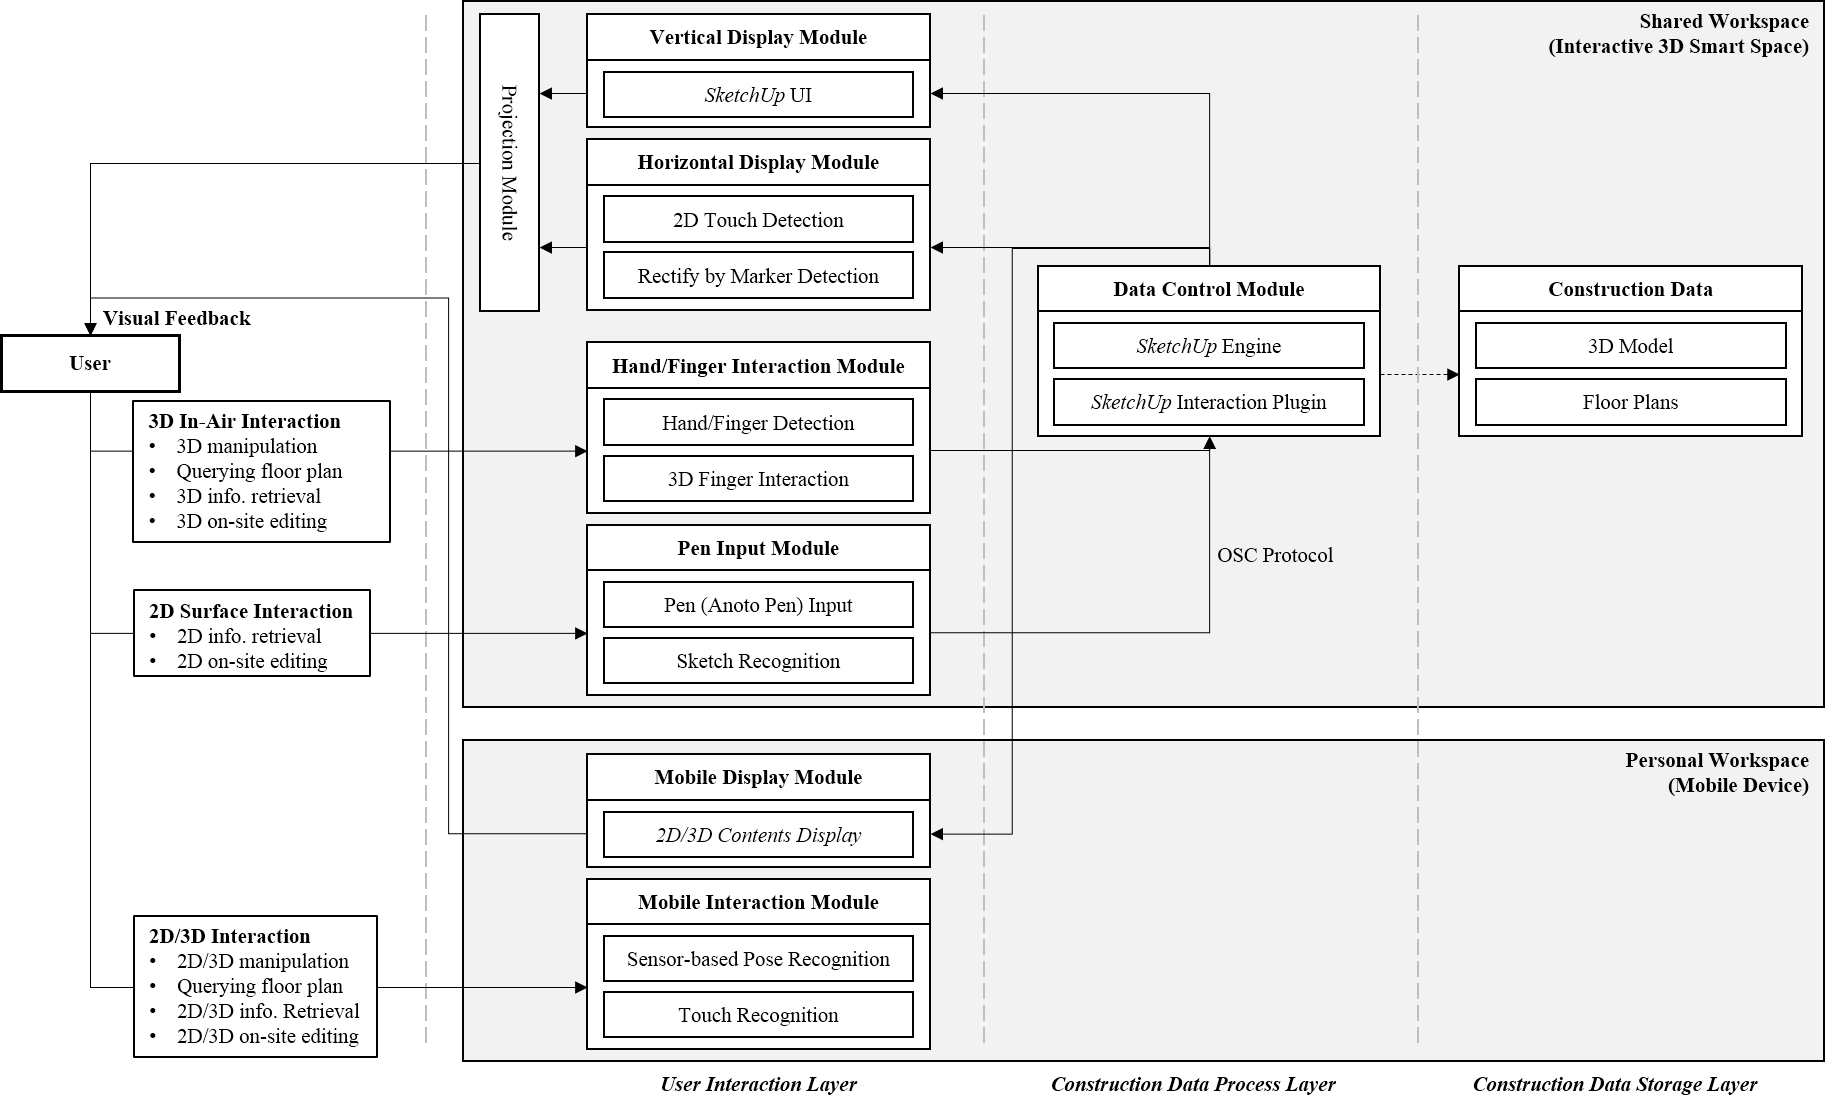
\includegraphics[width=1.0\textwidth]{3-System/system_components}
\caption{Software design of Proposed System}
\label{fig:overview}
\end{figure*}



% 한글버전
%!TEX root = ../Sensors_SmartConstruction.tex
% -*- root: ../Sensors_SmartConstruction.tex -*-

%\begin{comment}


%-----------------------------------------------------
\subsection{Computer Aided Construction}

\cite{harrison_architects_design_????}는 건축 공정을 예비설계, 건축 문서, 건축 관리의 3가지 단계로 구분하였다. IT 기술이 발전하면서 각 단계의 작업 효율성을 높이기 위한 다양한 연구들이 진행되고 있다.

첫번째 preliminary design phase는, architect가 자신의 conceptual design을 preliminary design으로 현실화(realize)하는 것을 도와주는 연구들이 진행되고 있다\cite{bae_ilovesketch:_2008, igarashi_teddy:_2007, song_modelcraft_2009, yu_prototype_2007, zeleznik_sketch:_2007}. 이러한 연구들은 기존 WIMP(Windows, Icons, Menus, Pointer)\cite{wikipedia_contributors_wimp_2014} 기반의 복잡한 인터페이스 대신 펜이나 손과 같은 Natural한 인터페이스를 사용한다. 이를 통하여 좀 더 빠르고 자연스럽게 프로토타이핑을 수행하여 architect가 drawing보다는 창의적인 컨셉 디자인에 집중할 수 있도록 한다. 

두번째 Construction documents를 위한 기술들은 Preliminary Design을 실제 건축에 사용될 수 있는 건축 문서로 변환하는 과정이다. 이러한 과정은 \textit{AutoCAD, 3dsMax, and SketchUp}과 같은 상용화 된 CAD software 들이 제공해주고 있다\cite{autodesk_3ds_????, autodesk_autocad_????, google_sketchup_????}.

세번째 Construction administration 영역의 연구는, 앞서 만들어진 건축 문서를 이용하여 건설 현장에 적용하는 과정을 보조하는 연구들이 진행되고 있다. 먼저 \cite{behzadan_enabling_2013, kim_interactive_2012} 연구들은 증강현실 기술을 이용하여 사전에 건축물이나 장비(equipments)들을 현장에 배치하여보고, 시뮬레이션을 제공하여 Conflict 등을 사전에 방지하는 연구들이 진행되었다. 이러한 연구들은 off-site에서 사전에 3D 객체를 manipulation하여 위험요소 등을 현실감 있게 고려(consider)할 수 있다는 장점이 있으나 실제 현장(in-site)에서 사용이 어렵다는 한계가 있다. 반면에 작업 현장에서 실시간으로 건축 정보에 접근하여 안전하고 정확한 시공을 제공하기 위한 연구들도 다양하게 진행되고 있다. \cite{aziz_supporting_2012, chen_framework_2011, giretti_design_2009}는 모바일 폰을 이용하여 필요한 정보를 즉시 접근할 수 있는 시스템 프레임워크를 설계하였다. 이러한 연구는 스마트 폰의 다양한 센서들을 Context Aware data로 사용하여, 건축 노동자가 필요한 정보를 적시에 제공할 수 있다. 하지만, 이러한 연구는 스마트 폰의 작은 인터페이스를 사용하기 때문에 3차원 데이터를 조작하기 어렵고, 양 손이 제한되며, 입력 인터페이스가 불편하여 현장에서으 피드백을 갱신하기 어렵다는 한계가 있었다. 이러한 시스템의 한계를 극복하기 위하여 \cite{behzadan_visualization_2005, khoury_high-precision_2009, yeh_-site_2012}는 Wearable Computing 기반의 방법으로 정보를 제공해주는 연구들이 진행되었다. Wearable Computing 기기를 사용하여 양 손이 자유로운 환경에서도 부가적인 정보를 얻을 수 있고 몰입도가 높아지는 장점이 있으나, 여전히 현장에서의 수정 사항 등을 반영하기 위한 인터페이스는 불편하거나 제공되지 않았다. Song, et al.\cite{song_penlight:_2009, song_mouselight:_2010}는 Interactive Surface 기술을 이용하여 입력 인터페이스 문제를 해결하였다. 이 연구에서는 Projector의 소형화를 예측하였고, 이를 통하여 펜에 부착 가능하거나 마우스 형태의 소형 프로젝터 컨셉을 제시하여 이러한 펜에 부착된 프로젝터를 이용하여 설계 도면의 정보를 획득하고 필요한 수정 사항 등을 갱신하도록 하였다. 하지만 이 연구는 2D surface에 국한되기 때문에 건축물의 3차원 정보를 획득하거나 접근하기가 어려웠다. 

%-----------------------------------------------------
\subsection{Interactive 3D Smart Surface}
Interactive Smart Surface 기술은 일반적으로 프로젝터와 카메라를 이용하여 일반적인 환경에 컴퓨터 기반의 Interactivity를 제공하는 기술이다\cite{kane_bonfire:_2009}. 프로젝터는 일상적인 환경에 Display 기능을 추가로 제공해주기 때문에 이러한 Interactive Smart Space를 구성하기에 적합하다. 이러한 연구는 Wellner's DigitalDesk\cite{wellner_digitaldesk_1991, wellner_interacting_1993}에서 시작하여 Augmented Surface\cite{rekimoto_augmented_1999}, EnhancedDesk\cite{koike_integrating_2001} 등의 다양한 연구가 진행되었다. 일반적으로 이러한 연구들은 고정형 프로젝터 환경에서 책이나 종이, 벽 등의 평면적인 대상들과 상호작용하는 연구들이 주로 이루어졌다. 

이후 Everywhere Display\cite{pinhanez_everywhere_2001, pinhanez_creating_2003, sukaviriya_portable_2004} 는 steerable projector를 설계하여 방 안의 여러 공간을 동적으로 사용할 수 있도록 제안되었다. 이러한 dynamic projection smart space 기술은 PlayAnywhere\cite{wilson_playanywhere:_2005} 시스템에서 모바일 형태로 발전되었다. 이 후 프로젝터 기기의 소형화로 handheld 크기의 프로젝터가 등장하면서 이러한 연구는 활성화되었다\cite{cao_interacting_2006, raskar_rfig_2004} 특히, PenLight\cite{song_penlight:_2009}는 펜에 부착 가능할 정도로 작은 프로젝터에 대한 비전을 제시하며 다양한 상호작용 방법을 제시하였다. 이러한 연구는 이 후에 다양한 펜 부착형 Smart Space 기술로 발전되었다. \cite{kim_ar_2013}는 이러한 portability를 이용하여 in-situ에서 designing을 위한 시나리오를 제안하였으며, \cite{kim_ar_2014}은 펜이 가장 많이 사용되는 학습 환경에 적용하여 학생들이 단지 펜만을 이용하여 Interactive Learning을 할 수 있는 시스템을 제안하였다. 이외에도 handheld 형태\cite{huber_lightbeam:_2012, kim_ilight:_2010}나 노트북에 embedded 형태\cite{kane_bonfire:_2009} 등 다양한 형태의 portable smart space 기술들이 등장하고 있다. 제안하는 Port3DAr 역시 건축 현장에서 사용하기 위하여 소형 portable 프로젝터를 사용하였으며, 편리한 거치를 위하여 tripod에 거치하는 형태로 설계하였다.

이러한 Smart Space 기술은 2D 평면에 한정된다는 한계가 존재한다. 최근의 여러 연구들은 이러한 제약을 벗어나 3차원 공간에서 Interactive Smart Space를 구현하기 위한 여러 연구들이 제안되고 있다\cite{grossman__2010}. 2차원 평면 위에서 3차원 컨텐츠를 제공하기 위하여 다양한 부가적인 기기를 이용하는 연구들이 진행되고 있으나 부피가 크고 복잡하다는 한계까 있으므로 건축현장에 적용하기에 어려움이 있다. 특히 Vertical Screen과 Horizontal Screen의 Dual Screen 기반의 시스템\cite{weiss_benddesk:_2010, coram_astrotouch:_2013, wimmer_curve:_2010, benko_miragetable:_2012}은 2차원 정보와 3차원 정보를 함께 제공할 수 있기 때문에 건축 현장에서 적용하기에 적합하다. 하지만 기존의 시스템은 vertical screen과 horizontal screen이 각각 독립적인 display로 구성되어 있었기에 부피가 크다는 문제가 있었으나, 제안하는 Port3DAr은 1대의 프로젝터 스크린을 'L'-shaped 공간에 프로젝션하여 공유하여 사용하기 때문에 portability를 높일 수 있었다.

최근의 Interactive Smart Space 기술은 \cite{jones_illumiroom:_2013, steimle_flexpad:_2013}와 같이 non-planar space에 projection되는 기술들이 연구되고 있다. 이러한 기술을 적용함으로써 복잡한 건축 환경에서도 적용할 수 있을 것으로 기대된다. 

%\end{comment}

% 영어버전
% %!TEX root = ../sigchi-sample.tex


\subsection{Computer Aided Construction}

\begin{comment}
In \cite{harrison_architects_design_????}, the construction process was divided into three stages preliminary design, construction documents, and construction control. As IT technology has developed, various studies have been done to heighten work efficiency in these areas.

First, in the preliminary design phase, there have been studies conducted in helping architects to realize their own conceptual designs into preliminary designs \cite{bae_ilovesketch:_2008, igarashi_teddy:_2007, song_modelcraft_2009, yu_prototype_2007, zeleznik_sketch:_2007}.
These studies use natural interfaces like pens or hands instead of complex interfaces based on existing WIMP (Windows, Icons, Menus, and Pointer). Through them, by executing prototyping faster and more naturally, they allow architects to focus on creative concept design rather than the task of drawing. 

Second, technologies for converting preliminary designs into construction documents have been studied and available in commercial computer-aided design (CAD) software like \textit{AutoCAD, 3dsMax, and SketchUp}.
%\cite{autodesk_3ds_????, autodesk_autocad_????, google_sketchup_????}.

Third, in studies of the construction administration area, using previously made construction documents, studies to aid the course of applying them to construction sites are being done. From studies \cite{behzadan_enabling_2013, kim_interactive_2012}, simulate the positioning of structures and equipment use at sites using augmented reality technology to prevent actual conflicts when structures are built physically.

These studies use 3D objects that are previously manipulated off-site and results from the simulation can detect risk elements realistically but this type of AR tool is not intended for on-site use. Other studies similarly have been used to provide safe and correct construction work based on real-time construction information at work sites. In \cite{chen_framework_2011, giretti_design_2009}, system frameworks were designed in order to access necessary information using mobile phones. These studies can provide necessary information of construction workers by using diverse sensors of smart phones as context aware data. But, these studies have limitations like difficulty in manipulating 3D data due to use of small interfaces of smart phones, restriction to both hands, and difficulty in feedback renewal from the inconvenience of the input interfaces. To overcome the system limits, studies to provide information by a method based on wearable computing were proposed as in \cite{behzadan_visualization_2005, khoury_high-precision_2009, yeh_-site_2012}.

In using wearable computing devices, there are big benefits that additional information can be gained in an environment giving freedom to use of both hands and an increased degree of immersion. However, interfaces to reflect amended matters on-site pose a challenge and previous methods have proved to be inconvenient or not available at all. Song, et al. \cite{song_penlight:_2009, song_mouselight:_2010} solved input interface problems using interactive surface technology. In the study, minimization of projectors was predicted and therefore, through it, by proposing a small projector concept possible to be attached to a pen or with a mouse type, using the projector attached to this pen, information of blueprints were made to be acquired and necessary amended matters were made to be renewed. Nonetheless, because this study is limited to 2D surface, it was difficult to get 3D information of structures or access them.
\end{comment}


The construction process was divided into three stages: preliminary design, construction documents, and construction control. As IT technology has developed, various studies have been conducted to increase work efficiency in these areas.

First, in the preliminary design phase, there have been studies conducted on helping architects to transform their conceptual designs into preliminary designs \cite{bae_ilovesketch:_2008, igarashi_teddy:_2007}. These studies use natural interfaces such as pens or hands, rather than complex interfaces based on windows, icons, menus, and pointer. By enabling faster and more natural prototyping and execution, these interfaces allow architects to focus on creative concept design, rather than the task of drawing.

Second, technologies for converting preliminary designs into construction documents have been studied and are available in commercial computer-aided design (CAD) software such as AutoCAD, 3dsMax, and SketchUp.

Third, in studies of construction administration, studies aimed at aiding in the use of applying previously created construction documents to construction sites are being conducted. Some studies \cite{behzadan_enabling_2013, kim_interactive_2012} simulate the positioning of structures and equipment use at sites using AR technology to prevent actual conflicts when structures are built physically.

These studies use 3D objects previously manipulated off site, and results from the simulation can detect risk elements realistically; however, this type of AR tool is not intended for on-site use. Other studies have been used similarly to provide safe and correct construction work based on real-time construction information at work sites. In \cite{chen_framework_2011, giretti_design_2009}, system frameworks were designed to access required information using mobile devices. These can provide required information regarding construction workers using diverse smart phone sensors as context-aware data. However, these studies have limitations, such as difficulty in manipulating 3D data owing to use of small smart phone interfaces, restriction to both hands, and difficulty in feedback renewal resulting from the inconvenience of the input interfaces. To overcome system limitations, studies of providing information using a method based on wearable computing have been proposed, as in \cite{behzadan_visualization_2005, yeh_-site_2012}.

Using wearable computing devices provides the substantial benefit that additional information can be gained in an environment with free use of both hands and increased immersion. However, interfaces for reflecting amended matters on site pose a challenge, and previous methods have proved to be inconvenient or unavailable. Song et al. \cite{song_penlight:_2009, song_mouselight:_2010} solved input interface problems using interactive surface technology. In that study, minimization of projectors was proposed, and using a small projector that could be attached to a pen or a mouse-type device enabled information regarding blueprints to be acquired and necessary changes to be renewed. Nonetheless, because this study was limited to 2D surfaces, it was difficult to get 3D information regarding the structures or to access them.


%%%%%%%%%%%%%%%%%%%%%%%%%%%%%%%%%%%%%%%%%%%%%%%%%%%%%%%%%%%%%%%%
%%%%%%%%%%%%%%%%%%%%%%%%%%%%%%%%%%%%%%%%%%%%%%%%%%%%%%%%%%%%%%%%
%%%%%%%%%%%%%%%%%%%%%%%%%%%%%%%%%%%%%%%%%%%%%%%%%%%%%%%%%%%%%%%%
%%%%%%%%%%%%%%%%%%%%%%%%%%%%%%%%%%%%%%%%%%%%%%%%%%%%%%%%%%%%%%%%
%%		Interactive 3D Smart Spaces

\subsection{Interactive 3D Smart Spaces}

\begin{comment}
Interactive "smart spaces" technology is a technology to provide computer-based interactivity to general environment normally by using a projector and a camera \cite{kane_bonfire:_2009}. Since a projector additionally provides the function of display to a user environment, it is an integral device in composing this interactive smart space. These kinds of studies started from Wellner's DigitalDesk \cite{wellner_digitaldesk_1991, wellner_interacting_1993}, and diverse studies like Augmented Surface \cite{rekimoto_augmented_1999} and Enhanced Desk \cite{koike_integrating_2001} were developed. Generally, in these studies, researches interacting with 2-dimentional objects like books, paper, walls, and so forth in fixed project environment were mostly realized.

Then, Everywhere Display \cite{pinhanez_everywhere_2001, pinhanez_creating_2003, sukaviriya_portable_2004} designed a steerable projector and proposed that several spaces in rooms could be used dynamically. This dynamic projection smart space technology has been developed into a mobile type in PlayAnywhere system \cite{wilson_playanywhere:_2005}. Later, owing to the minimization of projector devices and as a handheld-sized projector emerged these studies have been possible \cite{cao_interacting_2006, raskar_rfig_2004}. Especially, PenLight \cite{song_penlight:_2009} proposed various interaction methods while providing visions on small projectors to such an extent that it could be possible for them to attach to pens. These studies have later been developed into diverse pen-attached smart space technologies. \cite{kim_ar_2013} proposed a scenario for designing in-situ using this portability and \cite{kim_ar_2014} proposed a system that students can do interactive learning only with pens applying to a learning environment where pens are used mostly. Besides, diverse portable smart space technologies appear like the handheld type \cite{huber_lightbeam:_2012, kim_ilight:_2010} or an embedded type to notebook computers \cite{kane_bonfire:_2009}. The proposed Port3DAr also uses a small portable projector in order to be used at construction sites and was designed to be a standing type on a tripod for a convenient standing.

In these smart space technologies, the limit restricted to 2D plane exists. Recent studies have suggested methods to realize interactive smart spaces in 3D space without this restriction \cite{grossman__2010}. To provide 3D contents on 2D planes, studies [] using a number of additional devices have been developed, but because such systems used in those studies resulted in becoming bulky and complex, it is difficult to apply them to construction sites. In particular, developed systems like \cite{weiss_benddesk:_2010, coram_astrotouch:_2013, wimmer_curve:_2010, benko_miragetable:_2012} could be used on construction sites assuming the availability of dual displays for vertical and horizontal display which can provide 2D and 3D information together. However, because vertical and horizontal displays were composed as independent displays respectively in the existing system, there was a problem of its large bulkiness. Since the proposed Port3DAr uses one projector displayed onto an 'L'-shaped space to interact with shared content, portability can be heightened.

In recent interactive smart space technology, technologies like \cite{jones_illumiroom:_2013, steimle_flexpad:_2013} that can project onto non-planar spaces have been studied well for use in homes and offices but its use is equally applicable to scenarios in complex construction environments. 
\end{comment}


Interactive smart space technology provides computer-based interactivity to a general environment, typically using a projector and a camera \cite{kane_bonfire:_2009}. Since a projector provides the additional function of display to a user environment, it is integral to such an interactive smart space. These types of studies began with Wellner's DigitalDesk \cite{wellner_digitaldesk_1991, wellner_interacting_1993}, followed by diverse studies such as Augmented Surface \cite{rekimoto_augmented_1999} and Enhanced Desk \cite{koike_integrating_2001}. Generally, in these studies, research was conducted regarding interaction with 2D objects such as books, paper, and walls in a fixed project environment.

Subsequently, Everywhere Display \cite{pinhanez_everywhere_2001, sukaviriya_portable_2004} designed a steerable projector and proposed that several spaces in rooms could be used dynamically. This dynamic projection smart space technology has developed into a mobile form in the PlayAnywhere system \cite{wilson_playanywhere:_2005}. Later, owing to the minimization of projection devices and the emergence of handheld projectors, further studies have been possible \cite{cao_interacting_2006, raskar_rfig_2004}. In particular, PenLight \cite{song_penlight:_2009} proposed various interaction methods, while providing vision on small projectors to such an extent that they could be attached to pens. These have since been developed into diverse pen-attached smart space technologies. \cite{kim_ar_2013} proposed a scenario for designing in-situ using this portability, and \cite{kim_ar_2014} proposed a system that enables students to learn interactively using only pens in a learning environment where pens are primarily used. In addition, diverse portable smart space technologies, such as the hand-held type \cite{huber_lightbeam:_2012, kim_ilight:_2010} or the type embedded in notebook computers \cite{kane_bonfire:_2009}, have emerged. The proposed Port3DAr also includes a small portable projector to be used at construction sites and was designed to be a standing type on a tripod for convenience.

These smart space technologies are limited in being restricted to the 2D plane. Recent studies have suggested methods for creating interactive smart spaces in 3D space, without this restriction \cite{grossman__2010}. Studies using various additional devices have been developed to provide 3D content on 2D planes, but because the systems used in those studies are bulky and complex, it is difficult to apply them to construction sites. In particular, developed systems such as those described in \cite{benko_miragetable:_2012, weiss_benddesk:_2010, wimmer_curve:_2010} could be used on construction sites assuming the availability of dual displays for vertical and horizontal display that can provide 2D and 3D information together. However, because vertical and horizontal displays were created as independent displays in the existing systems, bulkiness was a problem. Because the proposed Port3DAr uses one projector displayed onto an L-shaped space to interact with shared content, portability can be increased.

In recent interactive smart space technology, technologies that can project onto non-planar spaces, such as those described in \cite{jones_illumiroom:_2013, steimle_flexpad:_2013}, have been studied extensively for use in homes and offices, but their use is equally applicable to scenarios in complex construction environments.






% end of Related Work
%--------------------------------------------------------------------------------------------



%!TEX root = ../construction.tex
% -*- root: ../construction.tex -*-

%!TEX root = ../construction.tex
% -*- root: ../construction.tex -*-

\section{Proposed System}


%%%%%%%%%%%%%%%%%%%%%%%%%%%%%%%%%%%%%%%%%%%%%%%%%%%%%%%%%%%%%%%%%%%%%%%
\subsection{System Overview}

\begin{figure}[ht!]
	\centering
    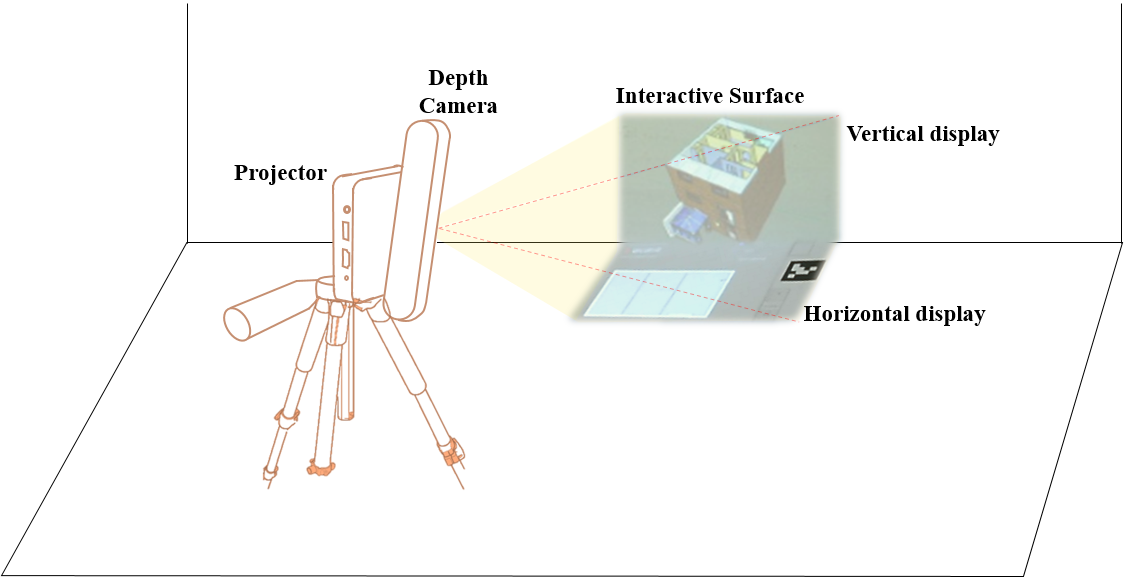
\includegraphics[width=0.8\textwidth]{3-System/overview}
	\caption{System Components}
    \label{fig:overview}
\end{figure}

제안하는 시스템은 전체적으로 그림 \ref{fig:overview}와 같이 구성된다. Interactive surface를 구성하기 위하여 한 쌍의 portable 프로젝터와 kinect 카메라 pair를 사용하였다. 이 portable 프로젝터를 통하여 현장에 필요한 정보를 제공할 수 있도록 하였다. 또한, Kinect 카메라를 이용하여 정보가 제공되는 공간을 인지함으로써 적합한 정보를 제공하거나 사용자와 상호작용할 수 있도록 하였다. 특히, 제안하는 시스템에서는 Horizontal Screen과 Vertical Screen을 구분하여 project 하도록 하였다. 이를 통하여 2차원 정보와 3차원 모델 정보를 동시에 제공함으로써 건축 현장에서 필요한 정보에 쉽게 접근하도록 하였다. Horizontal display에서는 도면위에 2D 정보를 projection 하며, Vertical display는 도면에 맞는 3D 모델을 출력한다. 두 개의 Display는 서로 동기화 되어 동작하며, 사용자는 직관적인 제스처 및 터치 상호작용을 통해 컨텐츠 제어가 가능하다.


%%%%%%%%%%%%%%%%%%%%%%%%%%%%%%%%%%%%%%%%%%%%%%%%%%%%%%%%%%%%%%%%%%%%%%%
\subsection{System Architecture}
\begin{figure}[ht!]
    \centering
    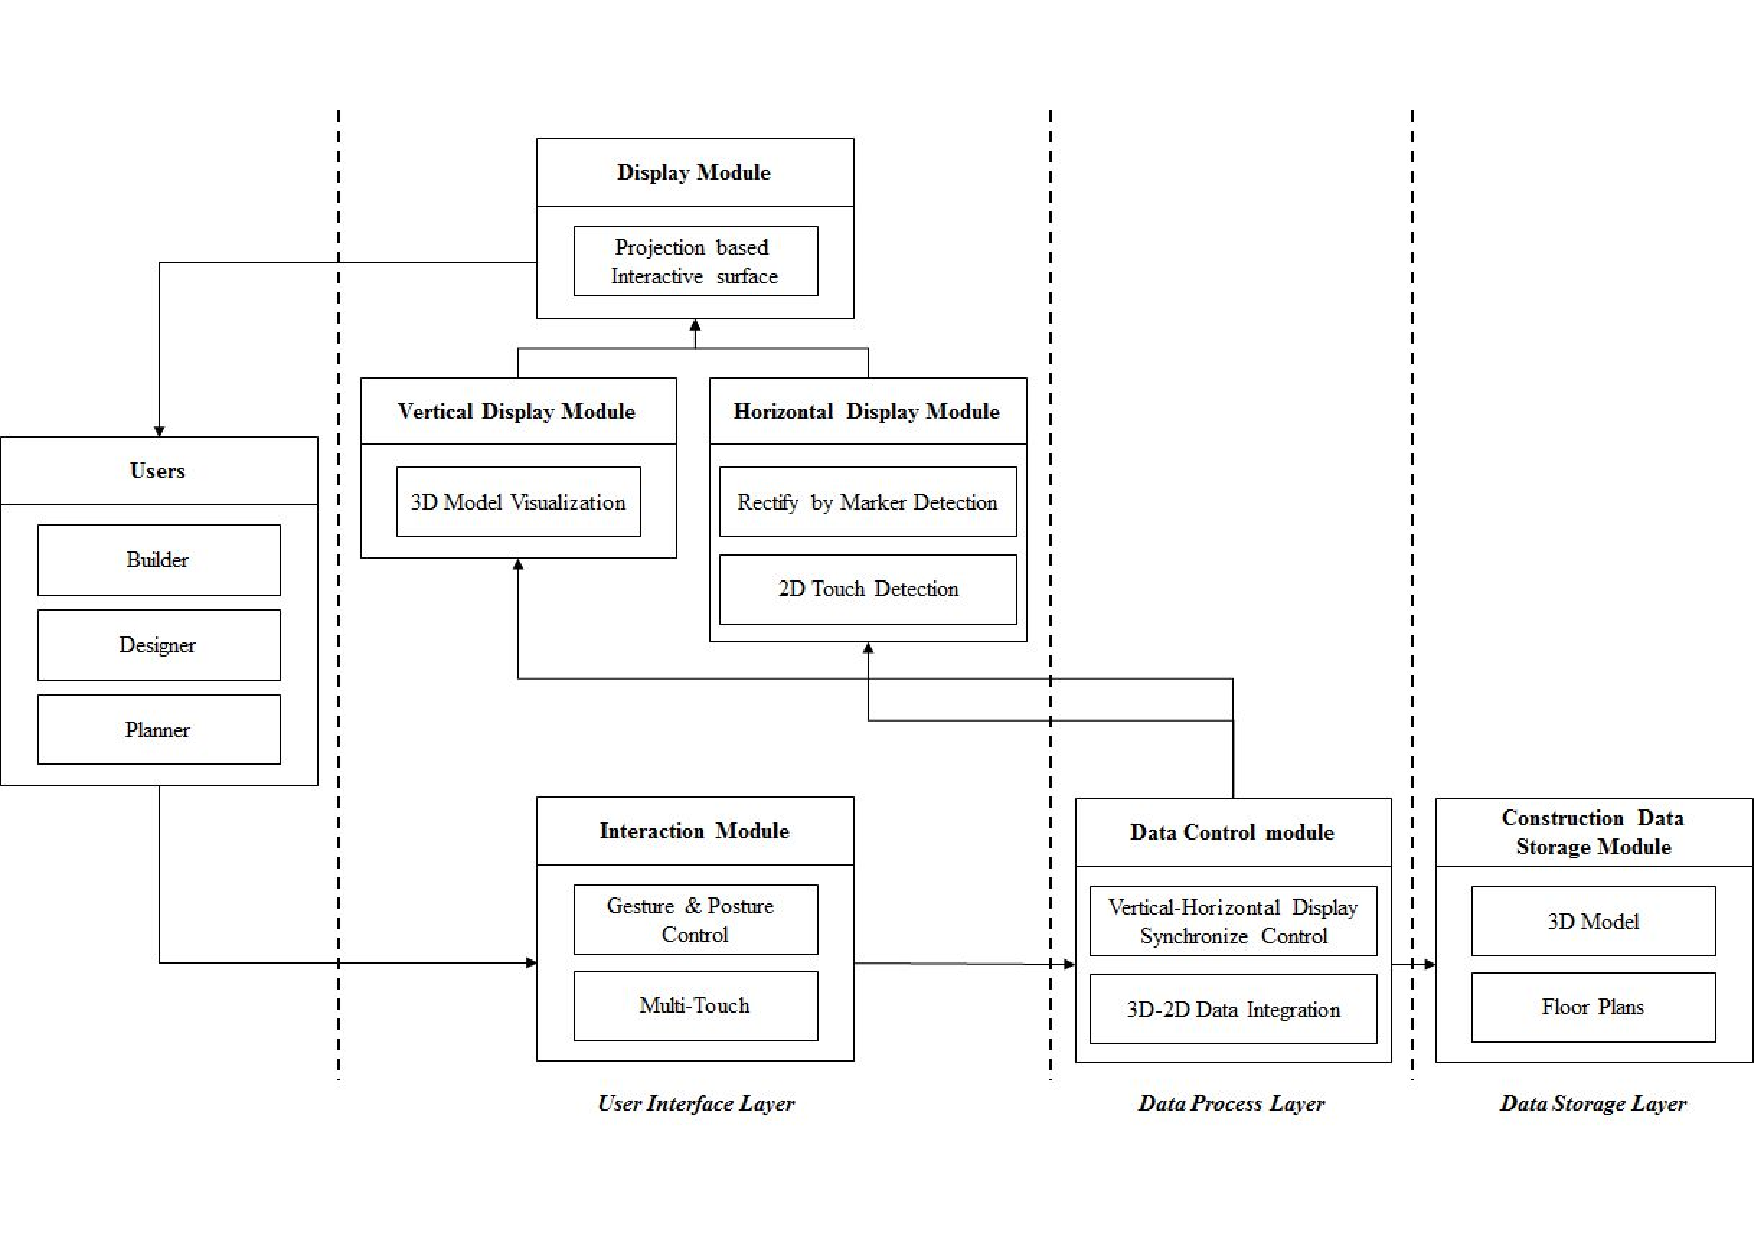
\includegraphics[width=\textwidth]{3-System/architecture_}
    \caption{The system architecture of proposed system}
    \label{fig:architecture}
\end{figure}



본 논문에서는 현장에서 필요한 정보를 이해하기 쉬운 형태로 제공하고, 현장 작업자들의 협업 지원을 위해 Projection 기반 시스템을 이용하여 시스템을 구성하였다.  Projection 기반인 Interactive Surface는 Vertical/Horizontal Display로 구성되며, 이를 이용하여 2D Floor Plan 과 3D 건축 모델의 정보를 제공한다. 또한 상호작용을 위해 제스처, 터치 기능을 지원함으로써 직관적인 제어가 가능하도록 하였다. 
그림 \ref{fig:architecture}에서 보듯이 시스템은 User Interface Layer, Data Process, Data Storage Layer 등 총 3개의 Layer로 구성되어 있다. 

\begin{itemize}
\item User Interface Layer : Vertical/Horizontal Display를 제스처, 터치 기능을 이용하여 직접적으로 제어 하며, 실시간 모델에 대한 상태 확인이 가능
\item Data Process Layer : 사용자가 입력한 건축 모델에 대한 제어를 인식하고, 결과를 Vertical/Horizontal Display에 실시간 반영하는 역할을 수행
\item Data storage Layer : 3D Model, Floor Plane와 같은 건축 정보 관리
\end{itemize}


%%%%%%%%%%%%%%%%%%%%%%%%%%%%%%%%%%%%%%%%%%%%%%%%%%%%%%%%%%%%%%%%%%%%%%%
\subsection{System Implementation}
\subsubsection{System Hardware / Hardware Implementation}
\begin{figure}[ht!]
	\centering
    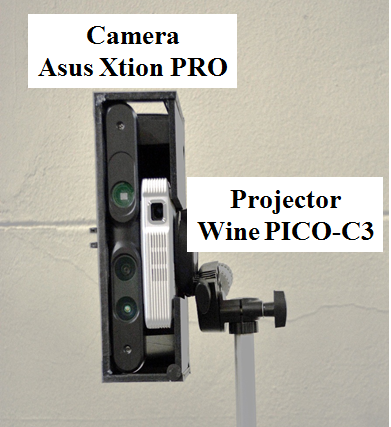
\includegraphics[width=0.4\textwidth]{3-System/hardware}
	\caption{Hardware Configuration}
    \label{fig:hardware}
\end{figure}
3D Interactive Surface의 구성을 위해 그림 \ref{fig:hardware}과 같이 Projection 기반의 하드웨어를 구성하였다. 본 연구에서 사용된 카메라는 Asus Xtion PRO, 프로젝터는 Wine PICO-C3를 사용하였으나, 다른 기종의 하드웨어를 사용하여도 무방하다. 카메라는 Horizontal Display 의 마커를 인식하고 사용자의 제스처와 터치를 인식하는데 사용되며, 프로젝터를 이용하여 영상을 출력한다. 인식하는데 카메라와 프로젝터는 캘리브레이션을 위해 서로 고정된 형태로 구성되어 있다. 이를 이용하여 마커를 인식하고, L-shape 벽면에 프로젝션 함으로써, 한 대의 프로젝터를 이용하여 Vertical/Horizontal Display 출력 및 제어가 가능하다.

%%%%%%%%%%%%%%%%
\subsubsection{Portable Multiscreen System}

제안하는 시스템은 2차원 데이터와 3차원 모델을 동시에 제공하기 위하여 Multiscreen interactive surface 기술을 이용하였다. 기존의 multiscreen interactive surface 기술은 display surface들이 고정되어 있었기 때문에 사전에 각 surface 사이의 위치 관계를 사전에 calibrate 하여 정보를 display할 수 있었다. 하지만, 제안하는 시스템은 Portable 환경을 지원하여야 하기 때문에 display surface들을 고정할 수 없고, 현장에서 즉각적으로 calibration 된 multiscreen을 제공하여야 하는 문제가 있었다. 따라서, 본 논문에서는 Image Marker 기술을 이용하여 Portable한 환경에서 실시간으로 screen을 calibrate하는 기술을 개발하였다.

\JHMEMO{calibration vs. distortion correction}

시스템의 calibration은 그림 \textcolor{red}{calibration 전/후 그림 삽입} 과 같이 Projector의 위치에 따라 찌그러져 project되는 영상을 rectify하는 기술이다. 본 논문에서는 그림 \JHMEMO{calibration 순서도 추가: 사전 calib, vertical calib, horizont calib} 와 같이 사전 Projector-Camera calibration과 Vertical Screen Calibration, Horizontal Screen Calibration 의 단계로 이루어진다. 

먼저, 사전에(offline으로) 카메라와 프로젝터 사이의 위치 관계를 보정한다. 그림 \JHMEMO{system 좌표관계 이미지}와 같이 제안하는 시스템은 IR 카메라와 RGB 카메라, 프로젝터로 구성된다. 이들은 각각 자신의 local 좌표계(coordinate system)를 가지고 있다. Offline calibration 단계에서는 이러한 센서의 intrinsic parameter와 extrinsic parameter를 계산함으로써 각 좌표계 사이에서 좌표를 변환할 수 있도록 한다. IR 카메라와 RGB 카메라 사이의 calibration은 Eq.\ref{eq:h_rgb2ir} 와 같이 checkerboard의 코너점을 각 카메라에서 인식하여 이 점의 correspondence를 계산함으로써 수행된다.
\begin{equation}
    P_{I} = H_{R \rightarrow I} P_{R}
    \label{eq:h_rgb2ir}
\end{equation}
여기에서 $P_{I}$와 $P_{R}$은 각각 IR 영상과 RGB에서의 대응된 checkerboard 코너점 집합을 의미하고, $H_{R \rightarrow I}$은 calibration결과 얻어진 RGB 영상의 좌표를 IR영상으로 변환하기 위한 행렬을 의미한다.
그리고 IR 카메라와 프로젝터 사이의 calibration은 그림 \JHMEMO{PROCAM Calibration 예제}와 같이 프로젝터로 빈 벽면에 checkboard image를 project하고 이를 RGB 좌표로 인식 한 후, 이를 IR 좌표로 변환하여 correspondence를 계산한다. 
\begin{equation}
\begin{split}
    P_{P} & = H_{R \rightarrow P} P_{R} \\
          & = H_{R \rightarrow P} H_{R \rightarrow I}^{-1} P_{I} \\
          & = H_{I \rightarrow P} P_{I}
    \label{eq:h_p2r}
\end{split}
\end{equation}
여기에서 $P_{P}$는 Projection 좌표계의 checkerboard점을 의미하고, $H_{R \rightarrow P}$와 $H_{I \rightarrow P}$는 RGB 영상과 IR 영상의 점을 Projection 이미지로 mapping 하는 변환 행렬을 의미한다. 이를 통하여 각각의 local 좌표계 좌표들은 서로 다른 좌표계로 쉽게 변환이 가능하고, 그림 \JHMEMO{calibration 결과: 손에 프로젝션 또는 checkerboard에 프로젝션}와 같이 영상을 인식하여 원하는 위치에 정보를 projection할 수 있다. 제안하는 시스템은 프로젝터와 카메라가 고정되어 있기 때문에, 이러한 프로젝터와 카메라 센서 사이의 calibration 과정은 off-line 프로세스로 단 한번만(only once) 수행된다. 

\begin{figure}[ht!]
    \centering
    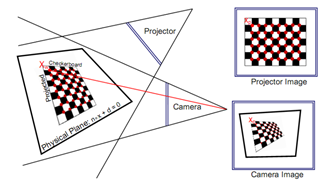
\includegraphics[width=0.4\textwidth]{3-System/calibration1}
    \caption{Projector-Camera Calibration}
    \label{fig:procam_calibration}
\end{figure}

이 후의 실시간 처리 단계에서는, projection 공간과 시스템의 위치를 분석하여 그림 \JHMEMO{rectified 결과 영상}과 같이 perspective distortion correction 을 수행한다. 이를 위하여 본 논문에서는 fiducial image marker를 이용한 distortion correction을 제안한다. fiducial image marker 는 그림 \JHMEMO{Fiducial Marker 설계}와 같이 미리 약속된 패턴의 이미지 태그이다. 미리 약속된 패턴을 인식하기 때문에, False Positive 가 낮고, ID와 pose 정보를 계산할 수 있다는 장점이 있다. 본 논문에서는 fiducial marker의 pose정보를 이용하여 distortion correction에 활용하였다. 먼저 아래와 같은 세 가지 제약사항을 가정한다.
%%% 제약사항
\begin{itemize}
    \item 프로젝션하고자 하는 평면은 평평함
    \item Fiducial marker는 직사각형
    \item Fiducial marker는 프로젝션 평면에 평행하게 위치함
\end{itemize}

가정 C3에 의하여 그림 \JHMEMO{Fiducial Marker 좌표계}에서 보는 것과 같이 Marker 좌표계는 World 좌표계와 평행하다. 
\begin{equation}
    P_M = kP_W
    \label{eq:marker2world}
\end{equation}
또한, C2에 의하여 Fiducial marker는 distortion되어 있지 않다. 따라서, Fiducial marker에 평행하게 정보를 projection하면 perspective distortion을 correct할 수 있으며, 이에 따라 marker에 평행한 Projection 좌표를 계산하는 것이 필요하다.
이는 앞의 식 \ref{eq:h_p2r} 을 이용하여 계산이 가능하다.
먼저 RGB 카메라를 이용하여 마커의 좌표를 인식한다.
\begin{equation}
    P_R' = \begin{pmatrix} 
        p_{R, 0}' \\
        p_{R, 1}' \\
        \vdots \\
        p_{R, n-1}'
    \end{pmatrix}
    \label{eq:marker2world}
\end{equation}
여기에서 







가정: 프로젝션 평면 위에 평행하게 놓임, 프로젝션 평면은 휘어있지 않고 반듯한 평면
$마커 좌표계 ~ k Projection World 좌표계$

Goal: Projection 좌표계가 나와야 함
프로세스:
  . 마커의 꼭지점 인식  
  . $마커 좌표계 - RGB 좌표계 간의 homography$
  . $마커 좌표계 ~ H R -> P  P    - projection 좌표계에 의한 마커 좌표계 계산$
  . $World 좌표계 ~ k 마커 좌표계 = H_R->P P$

\JHMEMO{predistorted 된 영상 추가}

Vertical vs. Horizontal
Vertical Screen은 고정되고, Horizontal Screen은 움직이면서 도면 제공
따라서 제안하는 시스템에서는 순서도에 따라 Vertical은 처음 1회 인식하고, Horizontal은 계속 인식함

이러한 Calibration 과정은 그림 \ref{fig:flowchart_calibration}와 같이, 사전 calibration과 realtime calibration으로 구분된다. 먼저, 사전 calibration 단계에서는, 카메라와 프로젝터 사이의 위치 관계를 보정한다. 이를 통하여 카메라를 통하여 입력되는 interactive space 에 정확하게 영상을 projection할 수 있도록 한다. 

\JHMEMO{Horizontally rotated image} 추가!

이 기술을 응용하여 MEP 정보 제공에도 사용함.
이는 벽면 등에 부착된 마커를 인식하여 Horizontal Marker 인식 모드로 진입하여 정보를 계속 제공함. (MEP 제공 영상)
























\begin{figure}[ht!]
	\centering
    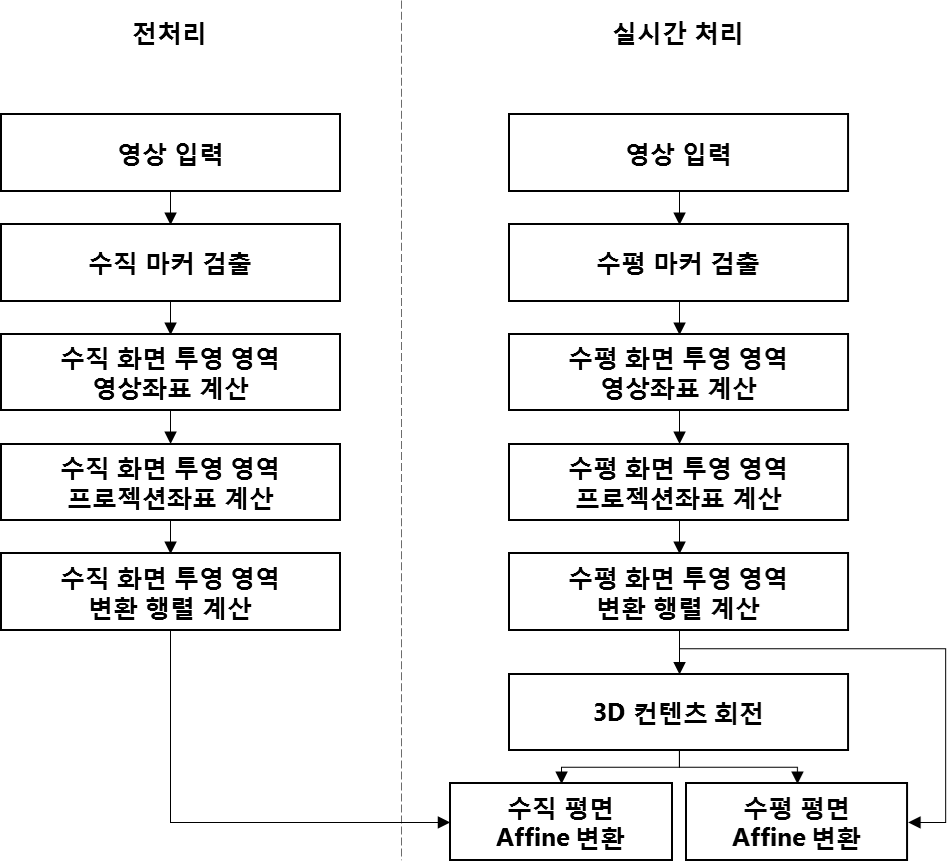
\includegraphics[width=1.0\textwidth]{3-System/flowchart_calibration}
	\caption{Calibration Flow Chart}
    \label{fig:flowchart_calibration}
\end{figure}


이 후 그림 \ref{fig:multiscreen_calibration}와 같이 Horizontal screen과 vertical screen 간의 multiscreen calibration은 마커를 이용하여 위치를 추정하였다. 
\begin{figure*}[!ht]
	\centering
        \begin{subfigure}[b]{0.8\textwidth}
            \centering
           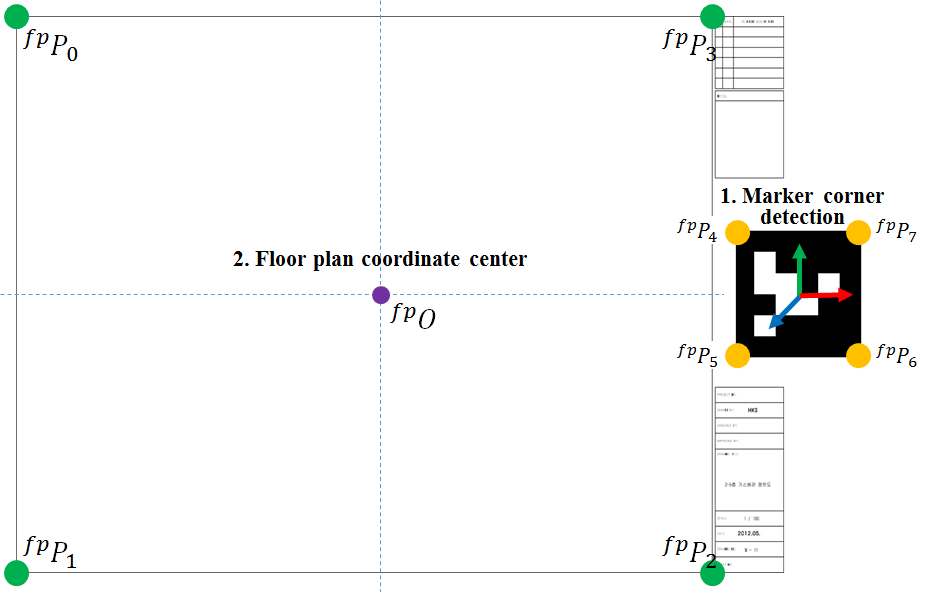
\includegraphics[width=\textwidth]{3-System/marker_calibration1}
                \caption{}
                \label{fig:marker_1}
        \end{subfigure}
        \\
        \begin{subfigure}[b]{0.8\textwidth}
	        \centering
              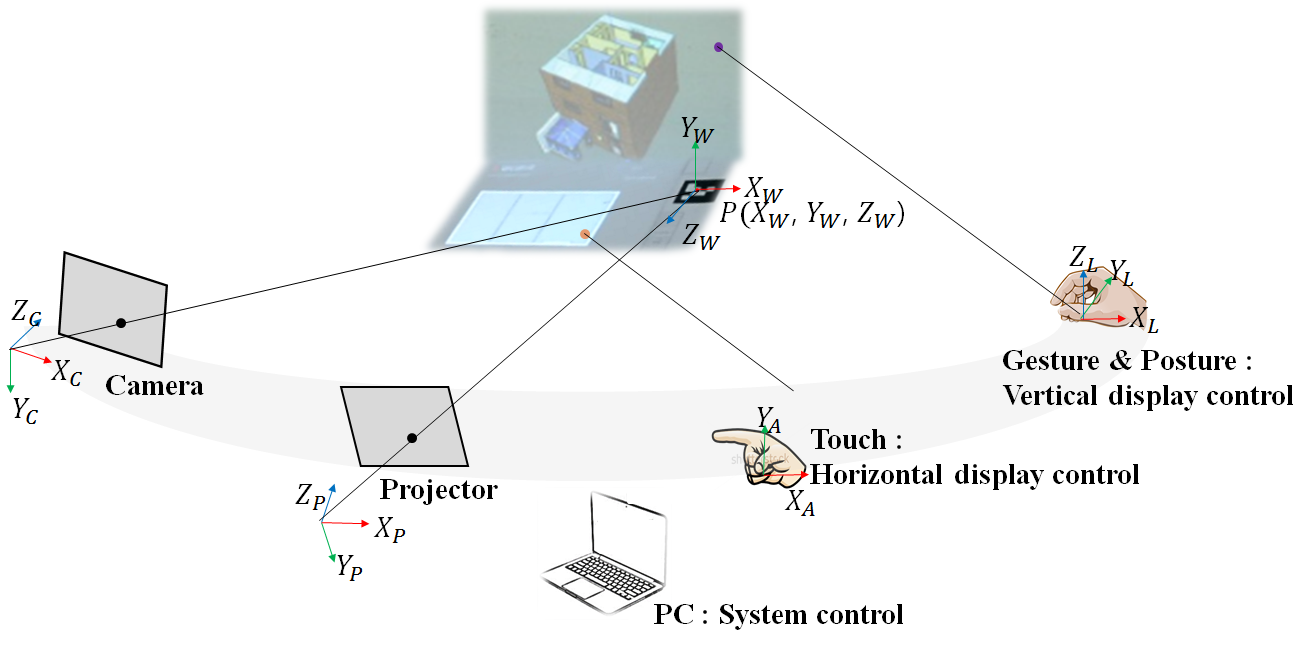
\includegraphics[width=\columnwidth]{3-System/marker_calibration2}
              \caption{}
              \label{fig:hardware}
        \end{subfigure}%
	\caption{Multiscreen Calibration}
    \label{fig:multiscreen_calibration}
\end{figure*}


위에서 설명한 캘리브레이션을 수행하게 되면 프로젝션을 위한 Vertical/Horizontal Display에 대한 위치가 결정 된다. 이러한 시스템을 이용하여 실시간 위치 추정이 가능하며, Portable 환경에서 한 대의 프로젝터를 이용하여 Multi-view를 생성하는 것을 가능하게 한다. 그림 \ref{fig:marker_calibration}은 실제 캘리브레이션을 수행하고, 마커를 이용하여 Vertical/Horizontal Display의 위치를 추정하는 단계이다. 
\begin{figure}[ht!]
	\centering
    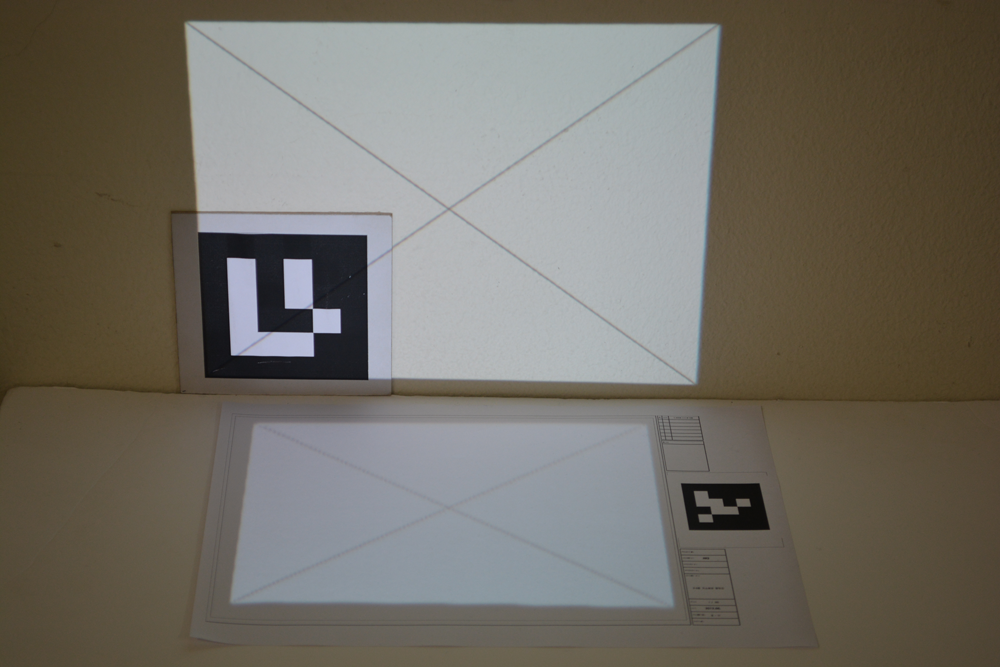
\includegraphics[width=\textwidth]{3-System/rectified}
	\caption{Marker-based Calibration}
    \label{fig:marker_calibration}
\end{figure}
입력된 영상을 기반으로 Vertical/Horizontal Display에 설정에 대한 전체적인 Flowchart는 다음과 같다. 
\textcolor{red}{Calibration Flowchart 삽입}

%%%%%%%%%%%%%%%%
\subsubsection{System Data Flow}
%%% 윤식!!! %%%





%!TEX root = ../construction.tex
% -*- root: ../construction.tex -*-

%%%%%%%%%%%%%%%%
\section{Application}


본 연구에서는 건축현장에서 프로젝션 화면을 이용하여 협업을 지원하고, 3D 모델 정보를 제공함으로써 원활한 정보공유가 가능한 시스템을 제안하였다. 시스템 검증을 위해 별도의 인터페이스 없이 상호작용이 가능한 터치 인식과 in-air 제스처 인식 기술을 이용하여 컨텐츠를 제공하였다. 사용자의 손 검출을 위해 깊이 영상을 이용한 거리 임계값 기반의 손 검출 알고리즘[ref]을 이용 하였으며, 손 동작을 인식하기 위해 Curvature[ref] 알고리즘을 이용하여 손의 포즈를 예측하였다. 
그림 0처럼, 실제 건축현장에 제안하는 시스템을 설치하여 어플리케이션 시나리오를 제공하였다. 'L'-shape의 바닥면인 Horizontal display의 2D 도면 마커를 인식하고 데이터베이스에 저장된 3D 모델정보를 Vertical display에 출력하여 Vertical display와 Horizontal display를 동기화 하였다. 동기화된 각각의 Display에 터치 인식 알고리즘을 적용하여 도면 및 특정 영역을 선택하고 이동시키는 것이 가능하며, 선택된 영역의 정보는 실시간 Display에 출력된다. 도면이 수정된 경우 자동으로 데이터베이스가 갱신되어 표현된다.  Horizontal display의 특정 영역을 선택한 경우 그림 1과 같이 표현되며, Vertical display을 터치 한 경우 그림 2와 같이 표현된다. 또한 양손의 위치정보를 이용하여 3D 모델의 확대/축소 및 회전 기능을 제공하였다. 그림 4에서 보여지는 것처럼, 양손의 위치정보를 이용하여 in-air 제스처 기반(그림 4.a)과 터치 인식 기반(그림 4.b)의 확대/축소 가 가능하다. 그림 5와 같이 양손의 위치정보와 방향성을 검사하여 Vertical display에 출력된 3D 모델의 회전제어도 가능하다.
추가적으로, 특정영역의 위치 추정을 위해 마커를 이용하고, 추정된 위치의 내부정보를 제공하기 위해 Mechanical Electrical and Plumbing(MEP) 정보를 프로젝션하는 컨텐츠도 제공하였다. 본 연구에서 제안된 정보는 그림6에서 보여지는 것처럼, 배관 정보만을 포함하고 있지만 배관, 배선 등 건물 외부 정보이외의 모든 내부 정보로 확대가능하다. 
제안하는 시스템 검증을 위해 제한적인 제스처 인식과 터치 인식을 이용하여 어플리케이션을 제공하였지만, 상호작용 기법은 추가 또는 변경될 수 있다.  






제안하는 연구는 프로젝션 화면을 이용하여 건축현장에서 협업을 지원하고, 정보공유를 원활 하게 한다. 또한 제공된 컨텐츠를 제어 및 수정하기 위해 다양한 상호작용 방법을 지원한다. 
\subsection{3D Model Manipulation}
설계도는 3차원 모델의 구조, 형상, 치수 등을 일정한 규약에 따라 2차원으로 투영하여 표현한 것이다. 제안하는 시스템은 2차원 설계도를 이용하여 3차원 모델의 정보를 현장에서 바로 확인할 수 있으며 제어 가능하다. 이를 위해 3차원 공간에서 손을 인식하는 NUI 기술을 통해 3차원 모델을 제어하고자 한다.
\begin{figure*}[!ht]
	\centering
        \begin{subfigure}[b]{0.32\textwidth}
	        \centering
                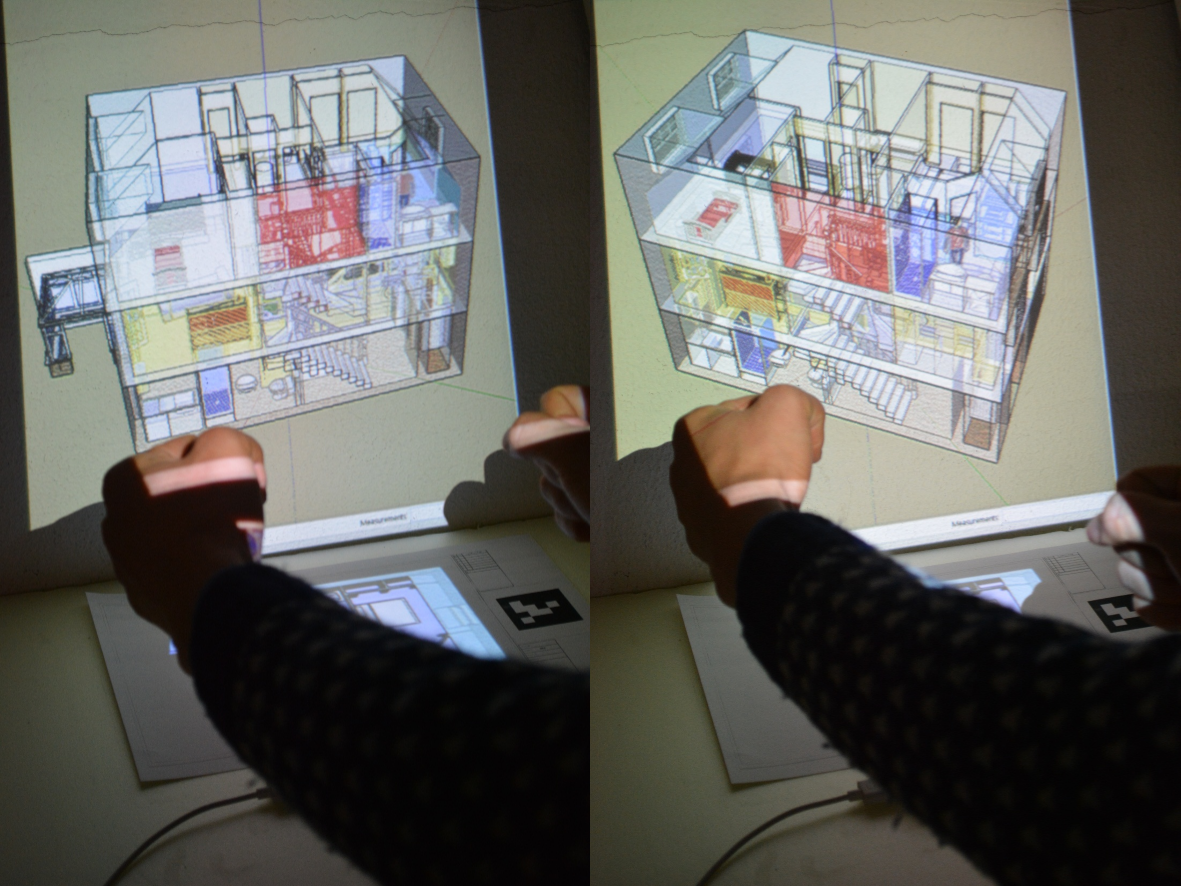
\includegraphics[width=\textwidth]{4-Interaction_Design/3d_rotate}
                \caption{Rotating the Model}
                \label{fig:rotate}
        \end{subfigure}%
        \hfill
        \begin{subfigure}[b]{0.32\textwidth}
            \centering
            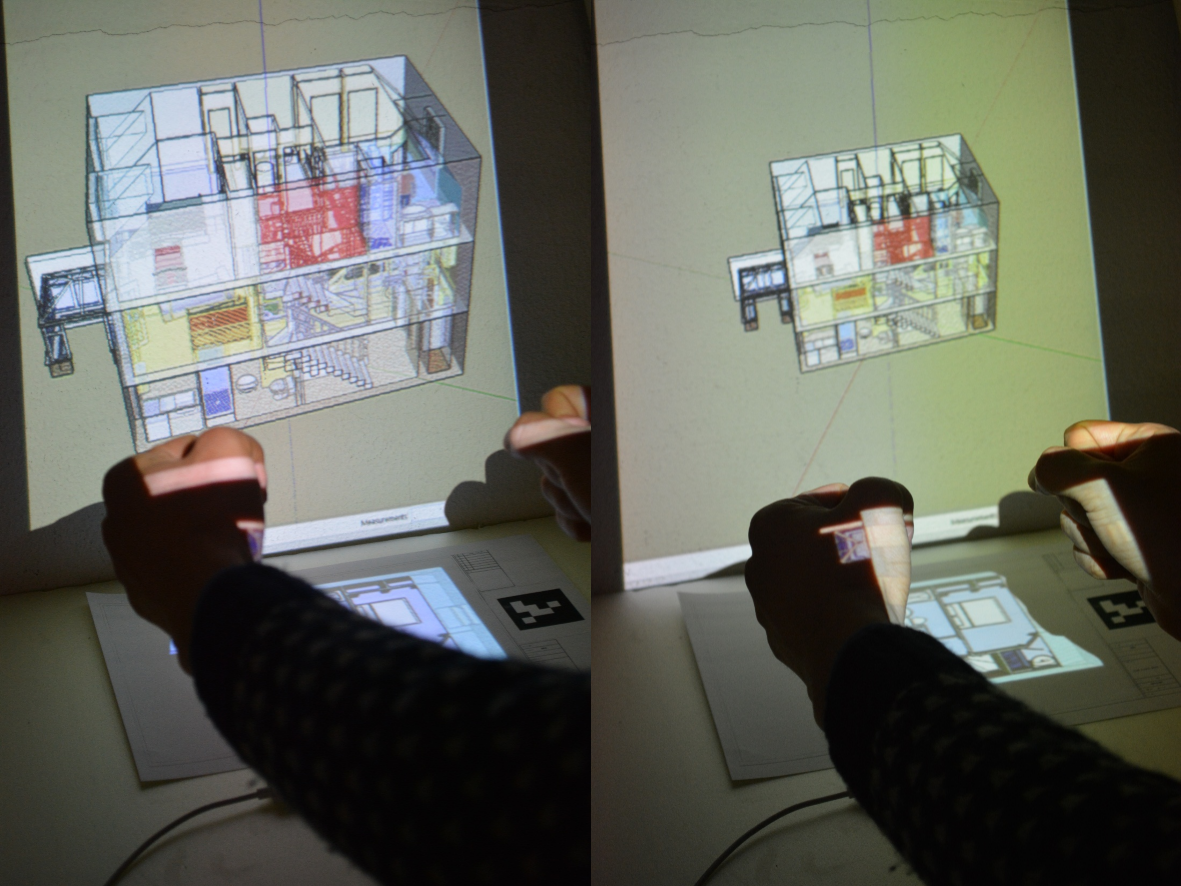
\includegraphics[width=\textwidth]{4-Interaction_Design/3d_scale_two_hand}
                \caption{Scaling by Two Hand Gesture}
                \label{fig:scale_two_hand}
        \end{subfigure}
        \hfill
        \begin{subfigure}[b]{0.32\textwidth}
            \centering
            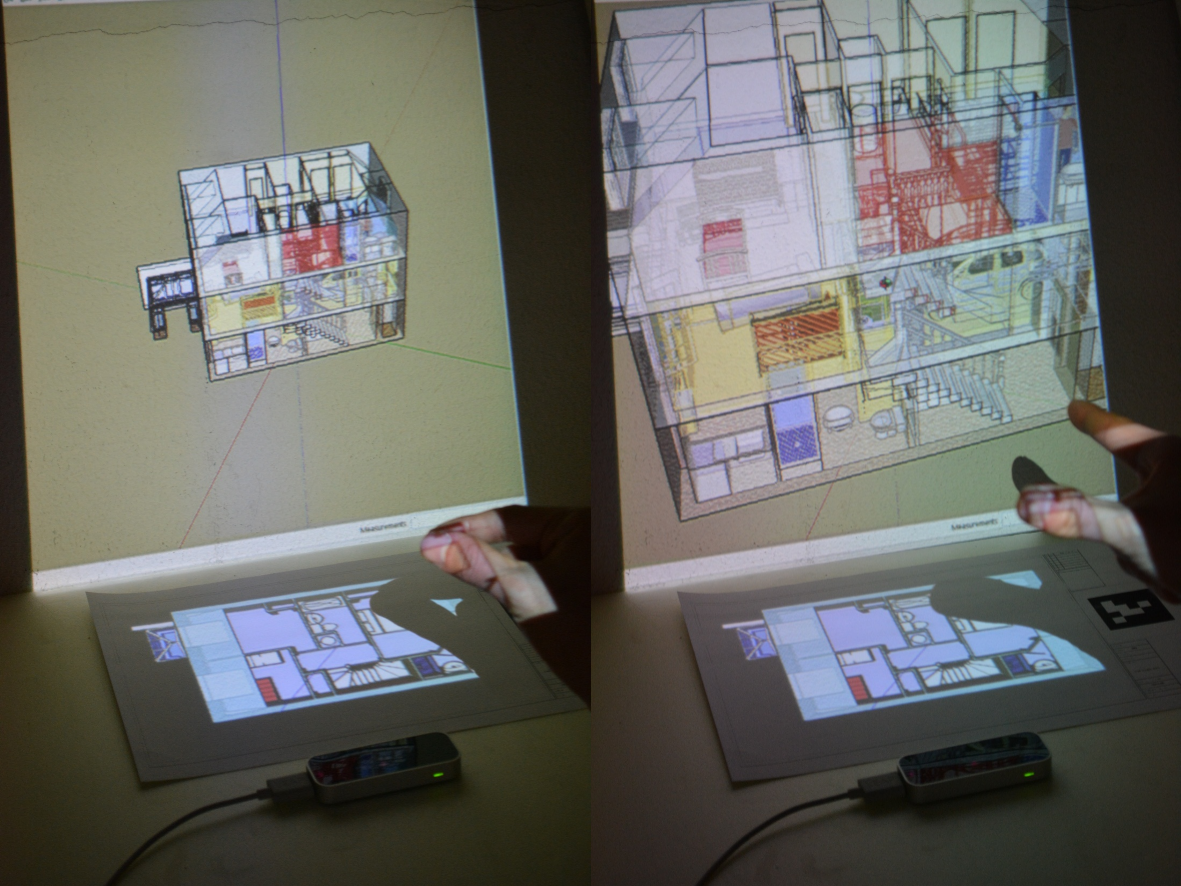
\includegraphics[width=\textwidth]{4-Interaction_Design/3d_scale_one_hand}
                \caption{Scaling by One Hand Gesture}
                \label{fig:scale_pinch}
        \end{subfigure}
	\caption{3D Manipulation}
    \label{fig:3d_mani}
\end{figure*}

사용자의 손 또는 손가락을 인식하여 3D 건축 모델의 회전 기능을 가능하게 한다. 그림 \ref{fig:rotate}처럼 사용자의 양손을 위치를 기준으로 3차원 공간에서 회전을 수행한다. 
Rotating 기능뿐만 아니라, 3D 모델을 확대하거나 축소하여 보는 Scaling 기능을 제공한다. 이 때, 직관적인 상호작용을 위하여 두 가지 모드의 Scaling 방법을 제공한다. 첫 번째 방법은, Rotating 기능과 동시에 수행할 수 있도록 양 손을 이용한 Scaling 기능을 수행 한다. 이는 그림 \ref{fig:scale_two_hand}과 같이 양손을 인식하고 거리 변화를 측정하여 3D 모델의 크기 조절을 가능하게 한다. 두 번째 방법은 그림 \ref{fig:scale_pinch}과 같이 손의 엄지와 검지 손가락을 이용하여 핀치 제스처를 인식하고 핀치 제스처의 움직임을 기반으로 3D 모델의 크기 조절이 가능하게 한다.

\subsection{Querying Specific Floor Plan}
특정 평면도의 정보에 접근할 필요가 있을 때, 그림 \ref{fig:layer}과 같이 손가락을 인식하여 평면도의 정보를 선택하여 확인 가능 하다. 시스템과 건축 모델링툴(ex, SketchUp)을 동기화하여 건물의 도면 정보를 이용하여 전체 건물 정보에서 특정 평면의 정보를 Horizontal Display에 증강 하도록 한다. 
 \begin{figure}[h!]
\centering
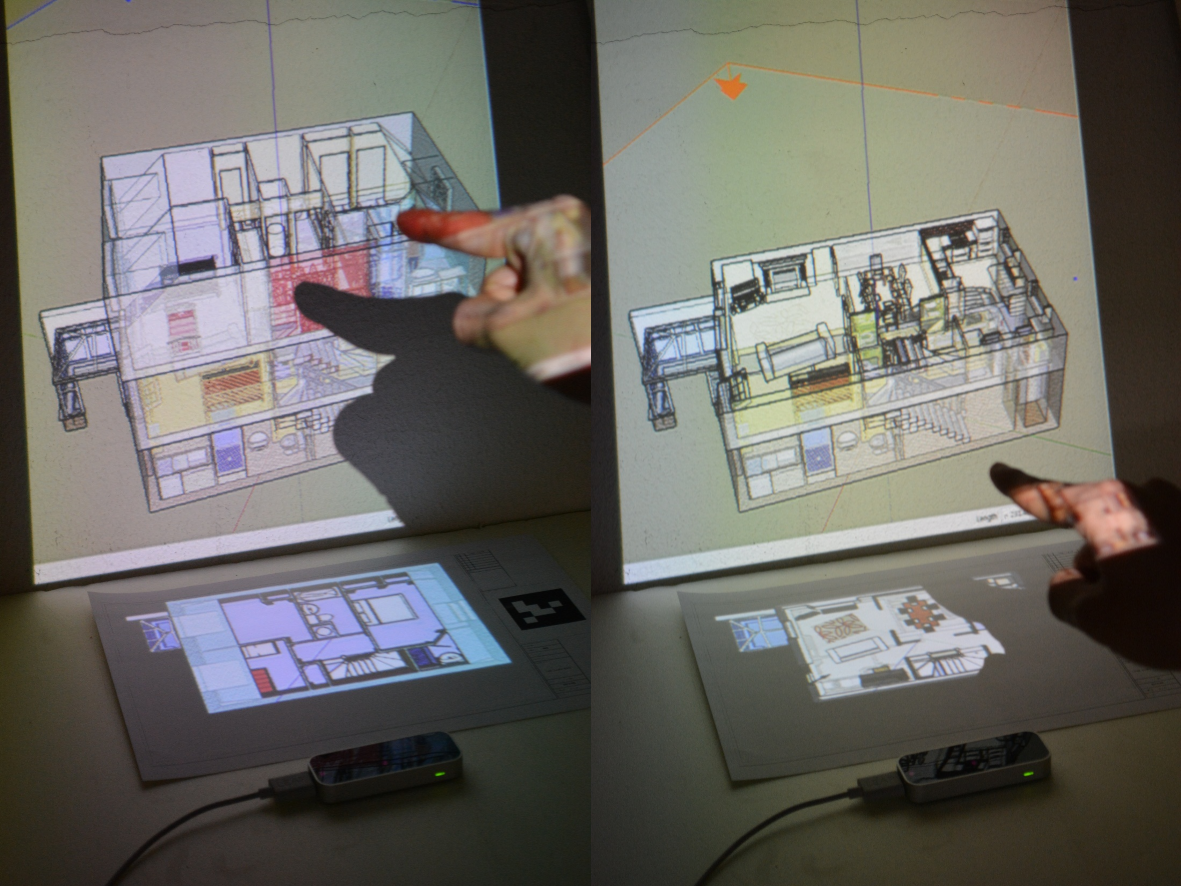
\includegraphics[width=0.4\textwidth]{4-Interaction_Design/query_plane}
\caption{Querying Specific Floor Plan}
\label{fig:layer}
\end{figure}


\subsection{Additional Information Retrieval}

또한, 취득한 도면의 부가적인 정보를 이용하여 면적이나 부피 등을 파악해야 하는 경우도 발생한다. 예를 들어 \cite{song_penlight:_2009}에서 제안한 것과 같이 건축 도면에서 부가적인 Dimension 정보를 제공하는 것은 현장에서 유용하게 사용될 수 있다. 본 연구에서는 건축 모델링툴 중 SketchUp에서 제공하는 Entity 정보를 이용하여 평면의 면적, 부피 등의 정보를 사용자에게 제공하였다. 또한 3D 정보를 제공함으로써 in-air 터치한 벽면의 넓이나 기둥의 높이 등의 3차원 Entity 정보를 제공할 수 있다. 
\begin{figure*}[!ht]
	\centering
        \begin{subfigure}[b]{0.55\textwidth}
	        \centering
                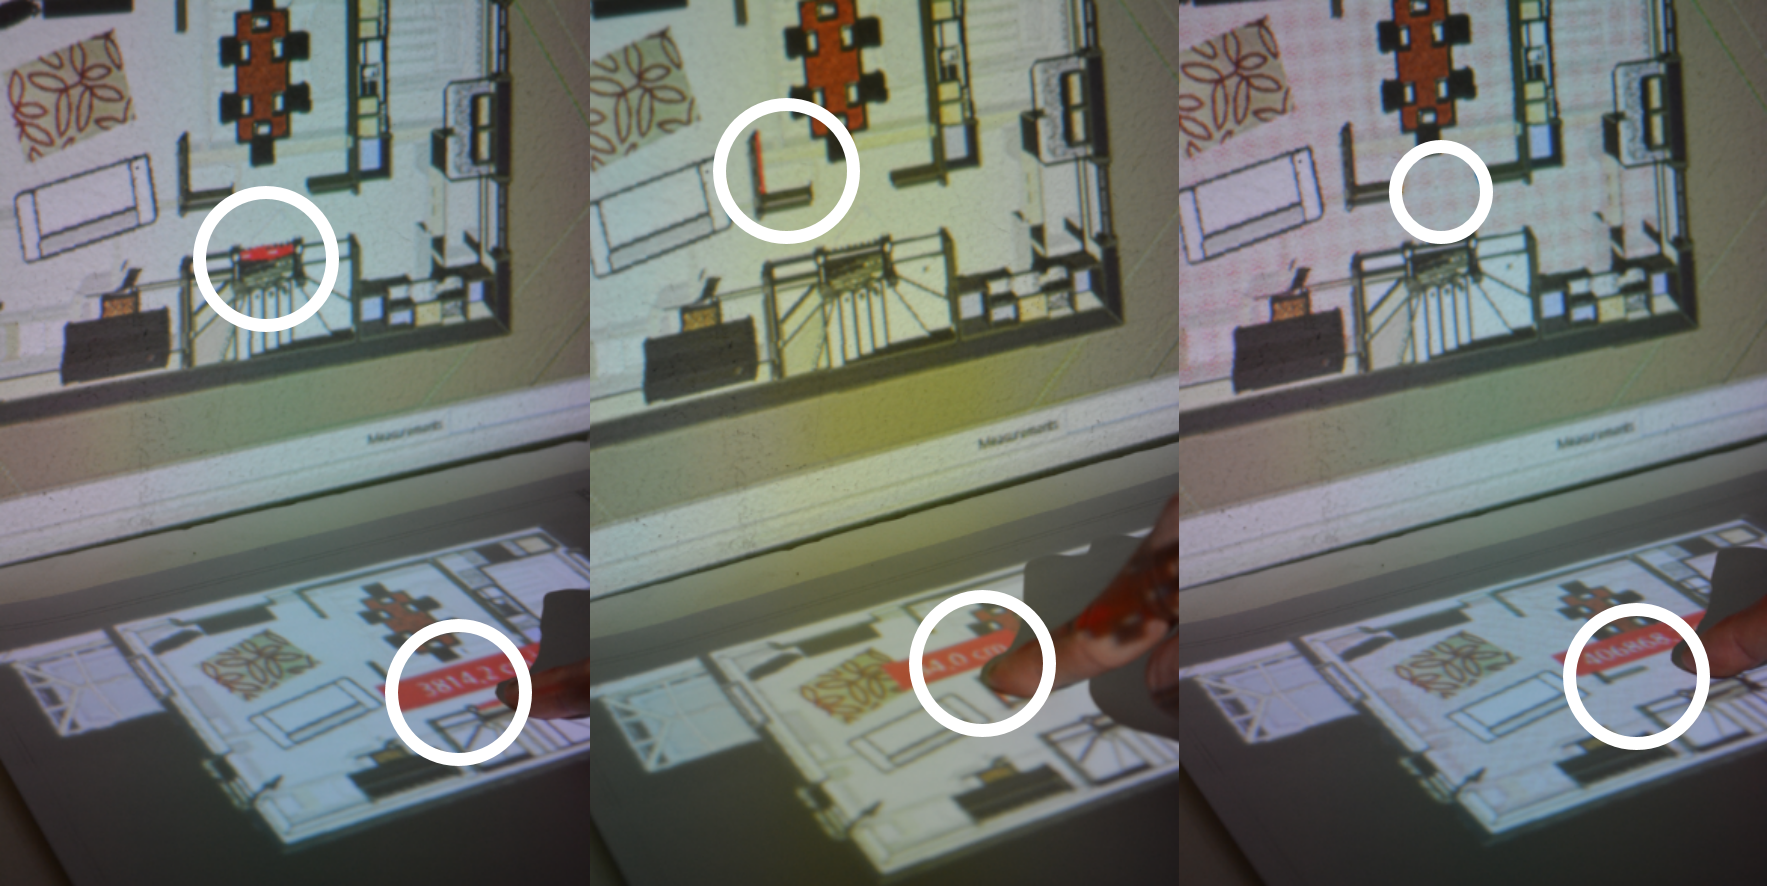
\includegraphics[width=\textwidth]{4-Interaction_Design/2d_info}
                \caption{Querying 2D information - length, area, volumn of specific entity}
                \label{fig:2d_info}
        \end{subfigure}%
        \hfill
        \begin{subfigure}[b]{0.37\textwidth}
            \centering
            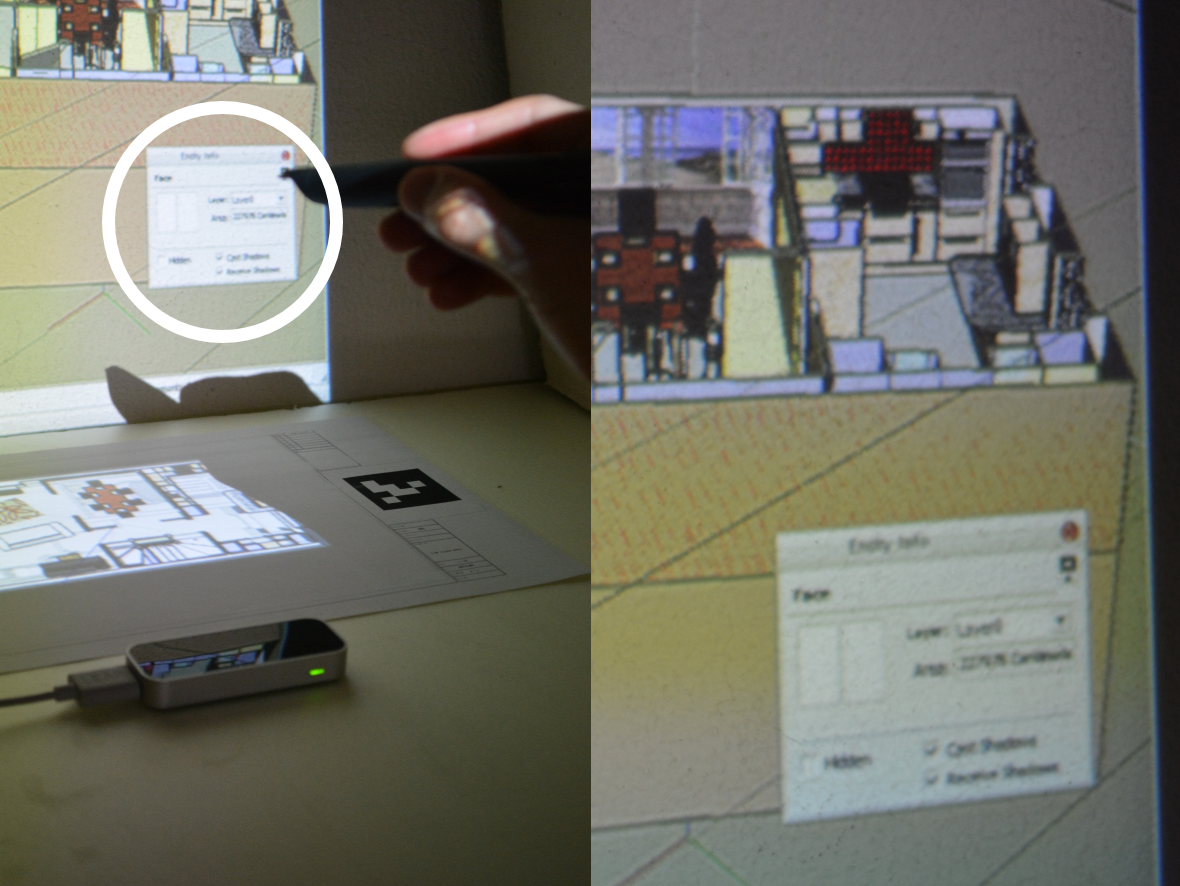
\includegraphics[width=\textwidth]{4-Interaction_Design/3d_info}
                \caption{3D information}
                \label{fig:3d_info}
        \end{subfigure}
	\caption{3D Manipulation}
    \label{fig:infor}
\end{figure*}


2D Information Retrieval
2D 정보 제공은 그림 \ref{fig:2d_info}와 같이 도면에 나타난 벽면의 길이나 바닥 면, 가구 등의 부피 등의 도면을 직접 터치함으로써 획득할 수 있다. 이는 해당 건축 도면 상에서 터치된 2차원 위치를 이용하여 시스템상의 Entity 정보를 이용하여 획득 가능하다.
3D Information Retrieval
3D 정보 제공은 그림 \ref{fig:3d_info}와 같이 제스처를 이용하여 3D 모델을 선택함으로써 정보를 제공받게 된다. 2D에 대한 정보 획득이 도면을 이용한 Horizontal Display를 이용한 입력이었다면, 3D에 대한 정보는 Vertical Display를 직접적으로 터치함으로써 입력이 제공된다. 

\subsection{On-site Editing}
현 시스템에서 도면의 변경이 필요한 경우, 정보에 대한 접근과 수정이 어렵기 때문에 변경사항을 실시간으로 반영하기 어렵다. 본 연구에서는 사용자의 손 움직임과 터치를 이용하여 건축 모델을 실시간 선택하고, 이동하거나 수정 가능하도록 하였다. 
\begin{figure}[h!]
    \centering
        \begin{subfigure}[b]{0.49\columnwidth}
            \centering
                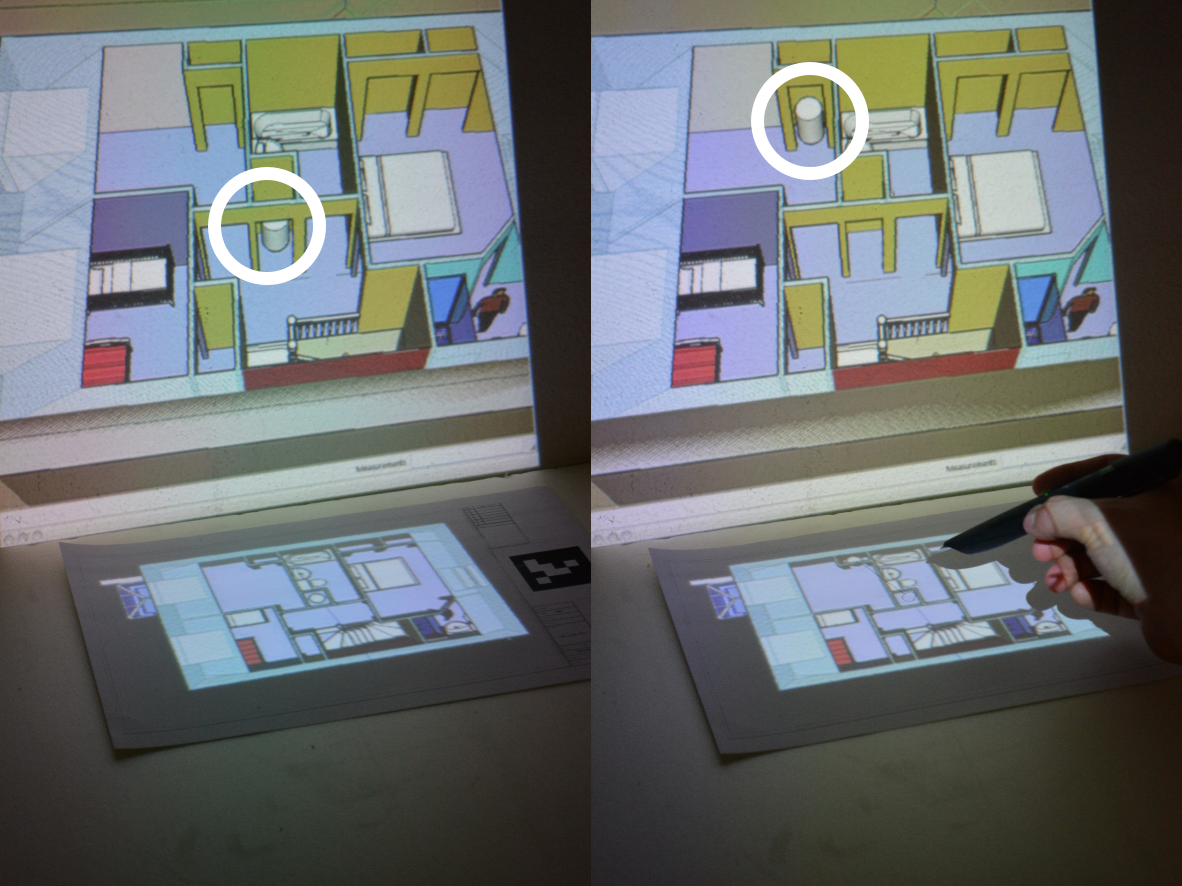
\includegraphics[width=1.0\columnwidth, height=3.6cm]{4-Interaction_Design/2d_move}
                \caption{Modifying 2D Entity using Pen}
                \label{fig:Pen_move}
        \end{subfigure}%
        \hfill
        \begin{subfigure}[b]{0.49\columnwidth}
            \centering
            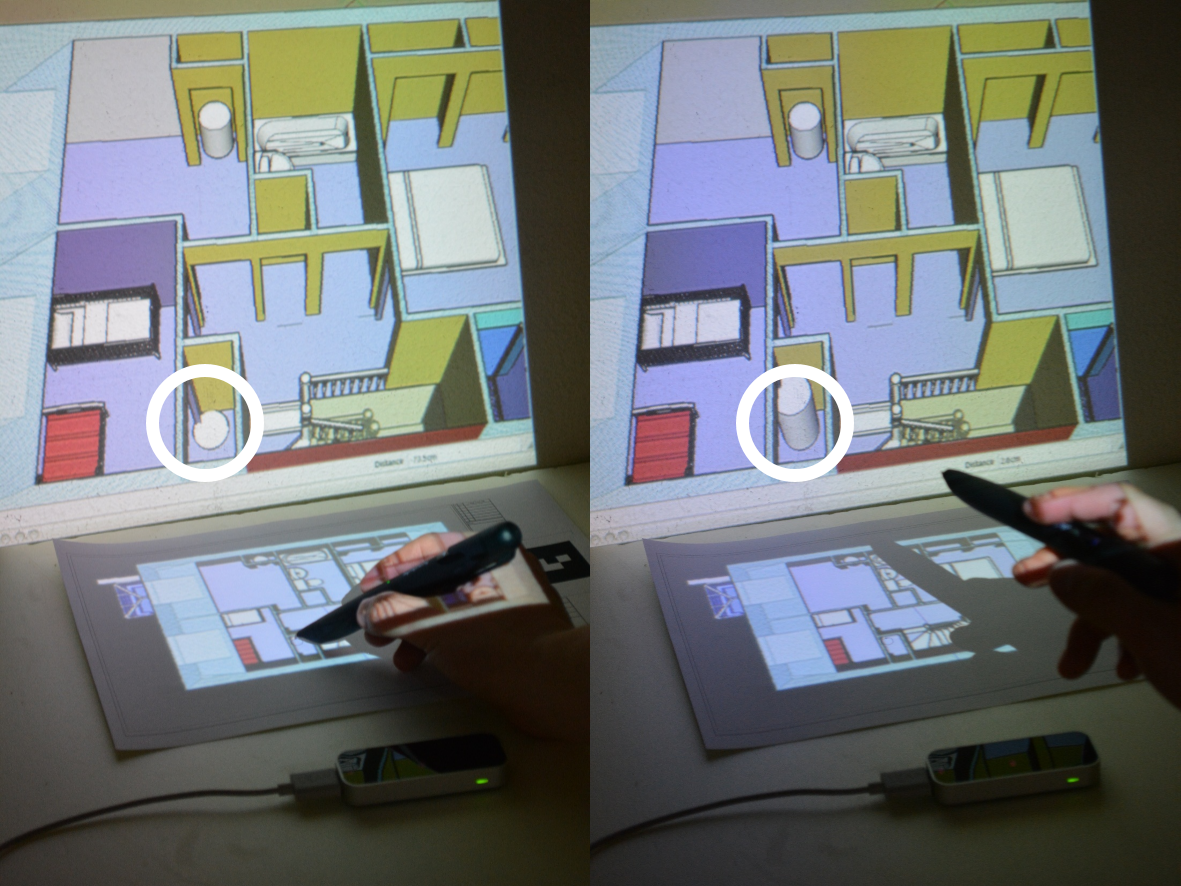
\includegraphics[width=1.0\columnwidth, height=3.6cm]{4-Interaction_Design/3d_note}
                \caption{Modifying 3D Entity in-air}
                \label{fig:Annotation}
        \end{subfigure}
    \caption{On-site Editing using Pen}
    \label{fig:edit}
\end{figure}

\textcolor{red}{제공된 컨텐츠를 정리하고, 전체적인 그림으로 표현, 삽입 예정}

%!TEX root = ../construction.tex
% -*- root: ../construction.tex -*-


%!TEX root = ../construction.tex
% -*- root: ../construction.tex -*-

\section{Experimental Result}

제안하는 시스템의 사용성과 효율성을 검증하기 위하여 사용자 테스트를 수행하였다. 실험은 \cite{yeh_-site_2012,lin_using_2014}를 참고하여 설계되었다.

\subsection{Demo Case}




\subsection{Experiments Design}

% 총 30~36명의 피실험자가 실험에 참여하였다. 이중 x명은 여자였고 x명은 남자가 참여했으며, 나이는 26세부터 43세까지이다. 피실험자의 x명은 civil engineering background이고 x명은 (construction professionals with experience in computer aided engineering, software development, structural analysis and design, construction planning, construction drawing, and project management.) 이들 대부분은 도면에 대한 이해도가 높고 CAD 프로그램에 대한 경험이 많았고, 또한 kinect등 제스처 기반 시스템에 대한 경험은 없었다. 

피실험자 설명 관련 설명: 인원, 성별 및 나이 구성, background

실험은 초반 15분 동안 demonstration session을 진행하였다. demonstration session 동안, 전체 시나리오에 대한 비디오를 보여준 후, 제안하는 시스템의 사용 방법에 대하여 설명하고, 나머지 시간 동안 실제로 사용해 본 수 있도록 하였다. 이후에 비교 실험과 사용성 평가를 실시하였다. 비교 실험은 \cite{yeh_-site_2012}과 마찬가지로 제안하는 시스템과 대조군 시스템 사이의 비교실험을 적용하여 몇 가지 과제를 수행하도록 하고 수행시간을 비교하였다. 모든 실험은 비디오로 녹화되었으며, 녹화된 동영상 분석을 통하여 수행시간을 측정하였다. 

대조군에 대한 설명 (paper 기반, 모바일, 제안하는 시스템)
모바일 앱
 - Autodesk® BIM 360 Glue
 - BIMx 

비교 실험에 수행된 과업은 \cite{yeh_-site_2012}와 유사하게 설계하여 실제 건축 환경에서 문제가 되는 task를 반영하였다. 이는 건축 현장에서 건축물의 정보를 획득하고 이를 다시 건축 모델에 반영하는 일련의 과정을 반영하고 있다. 세부적인 task는 아래와 같다. 각 task는 독립적으로 수행되었으며, 새로운 task 수행 전에 5분간의 휴식 시간을 제공하였다. 실험은 이러한 각 task의 수행 시간을 측정하였다. 
Random하게 수행하게 함

\begin{enumerate}
\item Exploration: 3차원 모델을 돌려보고 특정 뷰에 있는 특징 발견하기
\item Query: 특정 층의 특정 평면도 획득
\item Legend: 건축물의 평면도에서 특정 구조물의 dimension 획득
\item Modify: 건축물의 평면도에서 특정 구조물을 다른 위치로 이동됨을 표시
\item Discussion: 원격의 관리자와 건축물의 특정 위치의 이슈 에 대하여 의견 교환
\end{enumerate}

\begin{figure}[ht!]
	\centering
    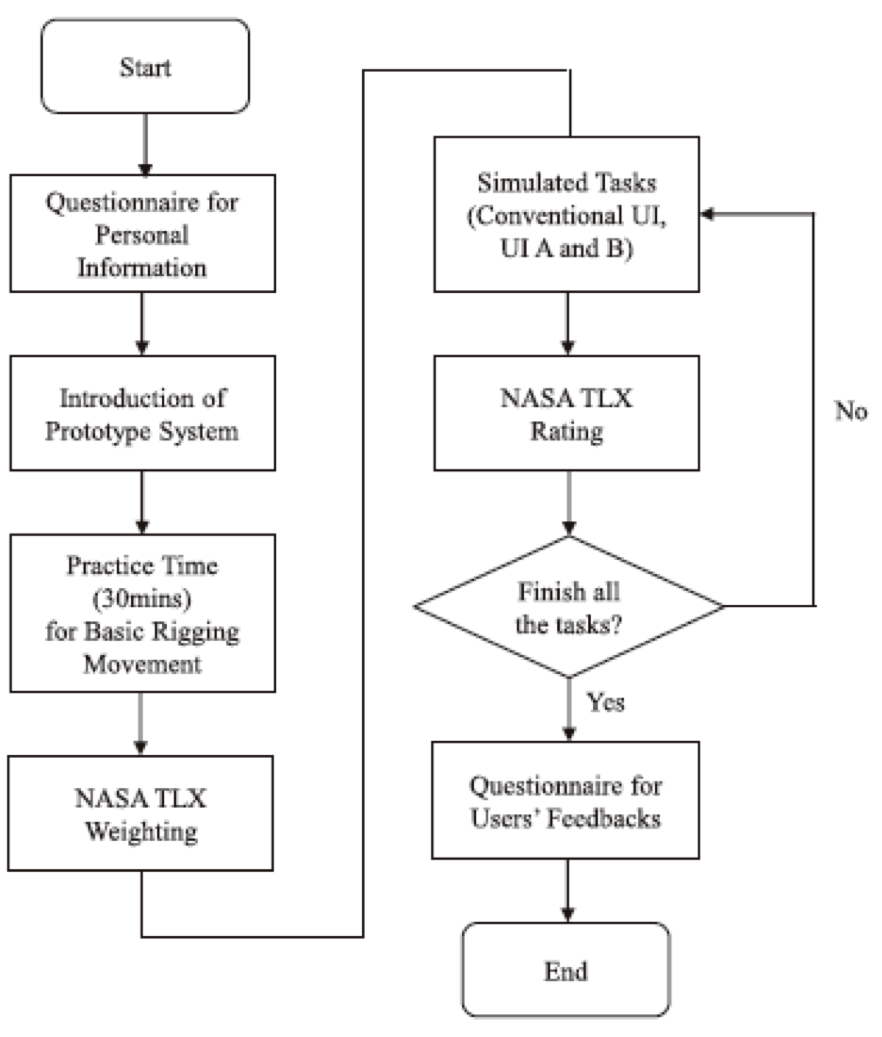
\includegraphics[width=0.4\textwidth]{5-Experiments/process}
	\caption{The process of experiments}
    \label{fig:exp_process}
\end{figure}

\ref{fig:exp_process} 와 같은 형태로 실험 단계 수행

\subsection{Efficiency}

Completion time, success rate test

\subsection{effectiveness}
Task loading score for participants (NASA Task Load indeX) test

\textit{
\begin{itemize}
\item Six weighted factors (Mental Demands, physical demands, temporal demands, effort, performance, frustration)
\item Mental Demand: How much mental and perceptual activity was required? Was the task easy or demanding, simple or complex?
\item Physical Demand: How much physical activity was required? Was the task easy or demanding, slack or strenuous?
\item Temporal Demand: How much time pressure did you feel due to the pace at which the tasks or task elements occurred? Was the pace slow or rapid?
\item Overall Performance: How successful were you in performing the task? How satisfied were you with your performance?
\item Frustration Level: How irritated, stressed, and annoyed versus content, relaxed, and complacent did you feel during the task?
\item Effort: How hard did you have to work (mentally and physically) to accomplish your level of performance?
\end{itemize}
}

\begin{figure}[ht!]
	\centering
    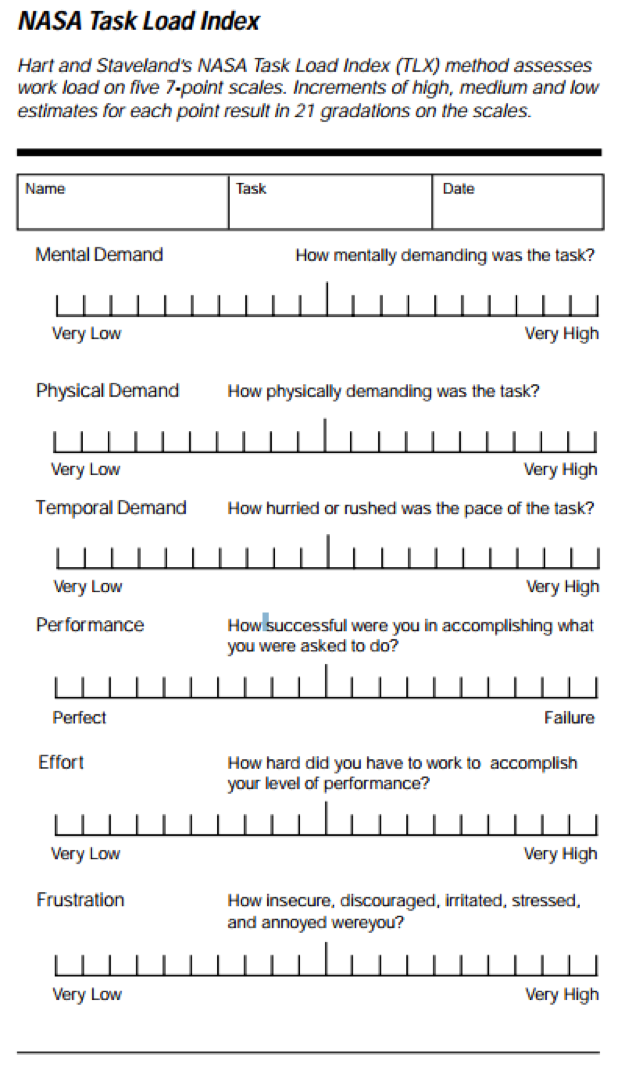
\includegraphics[width=0.4\textwidth]{5-Experiments/NASATLX}
	\caption{Questionnaire of NASA TLX}
    \label{fig:nasa_tlx}
\end{figure}

\subsection{usability}

Usability test (Perceived Usefulness and Usability)





%===============================================================================================
%	Experiments
%	목표 분량: 0.5장

%  \begin{figure*}[!t]
% \centering
% 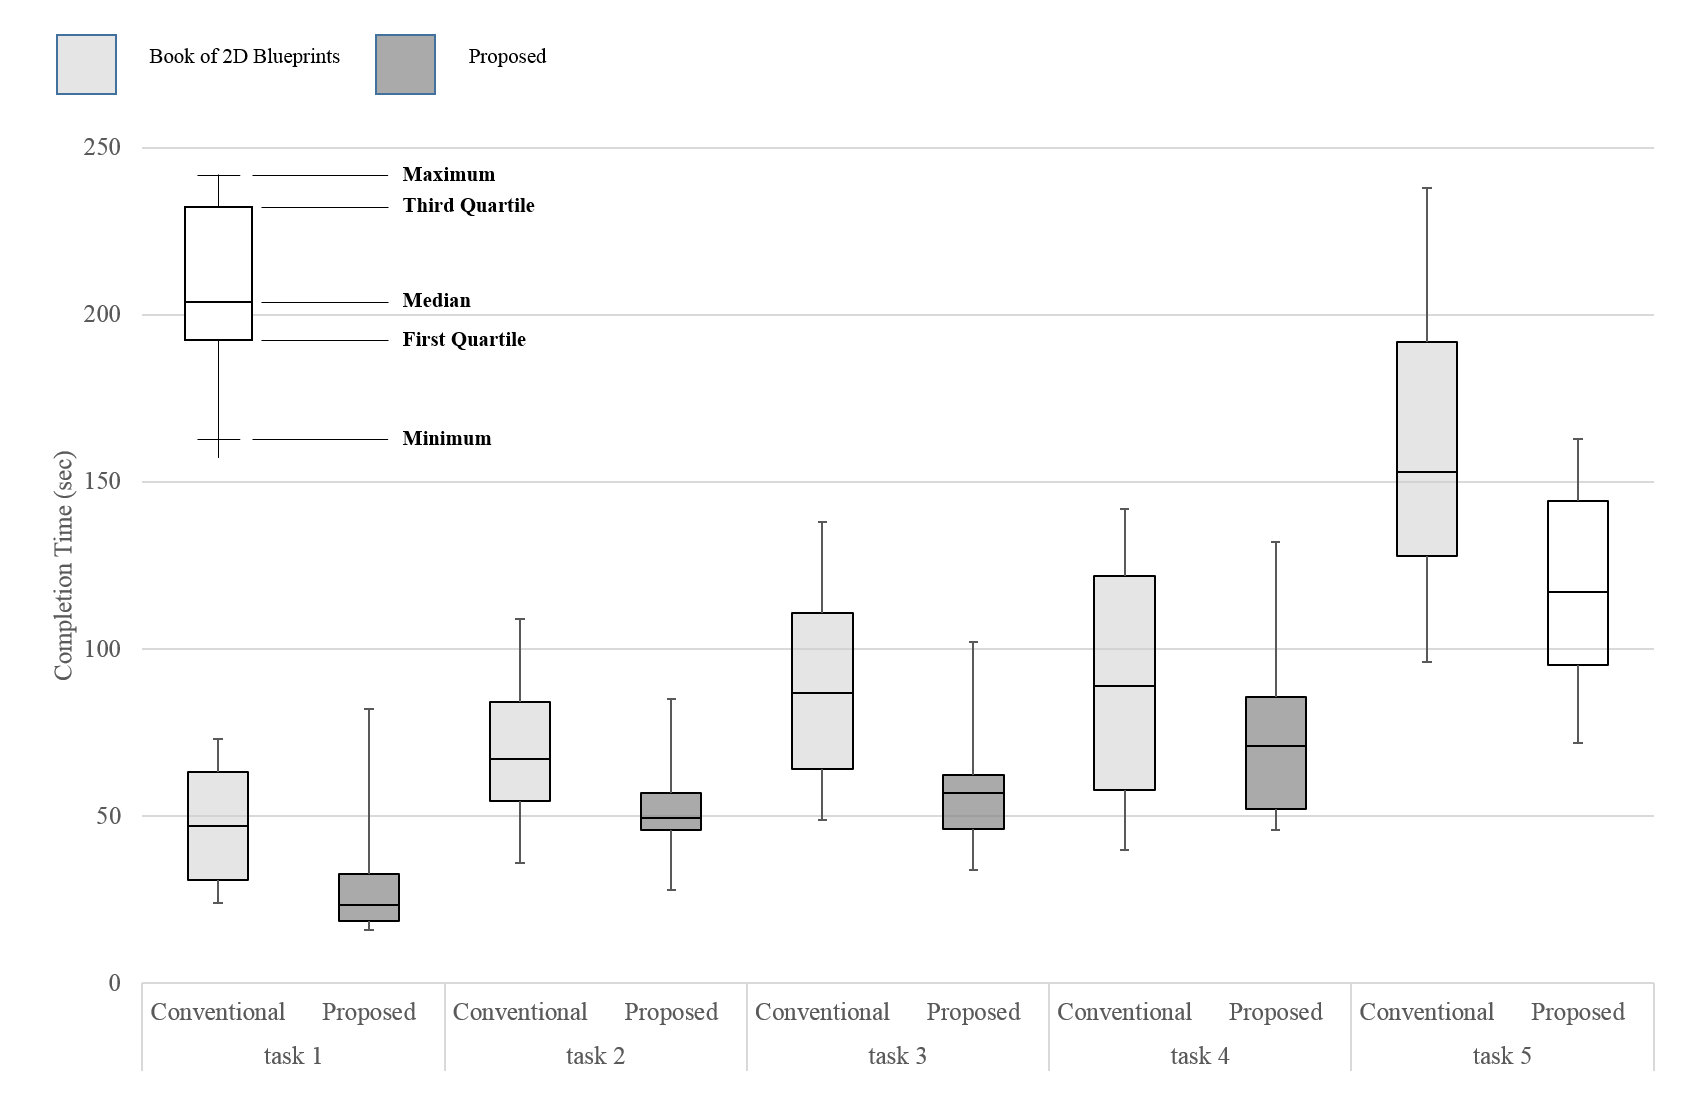
\includegraphics[width=0.8\textwidth, height=7.8cm]{5-Experiments/completion_time}
% \caption{Test completion time}
% \label{fig:completion_time}
% \end{figure*}

% \section{Experiments}
% % \begin{comment}
% 제안하는 시스템의 사용성을 검증하기 위하여 사용자 테스트를 수행하였다. 실험의 설계는 \cite{song_penlight:_2009, yeh_-site_2012}를 참고하여 설계되었다. %완료%


% 실험은 4가지 테스트 시나리오에 대하여 정량적 평가와 정성적 평가를 수행하였다. 그리고 semistructured interview 를 통하여 추가적인 comment와 insight를 얻을 수 있었다.   %수정?%
% % \end{comment}

% %% 번역 원본
% % To verify usability of the proposed system, a user test was executed. The experiment was conducted referring to \cite{song_penlight:_2009, yeh_-site_2012}. We executed a comparison test against conventional 2D drawing based approach, and took questionaire about perceived usefulness and ease of use. Then, through a semistructured interview, additional comments and insight could be gained.

% %% 번역 결과
% % A user test was conducted to verify usability of the proposed system, referring to \cite{song_penlight:_2009, yeh_-site_2012}. We conducted a comparison test against a conventional 2D drawing based approach and circulated questionnaires regarding perceived usefulness and ease of use. Then, additional comments and insight were obtained through semi-structured interviews.


% \subsection{Test Participants}
% % \begin{comment}
% 총 20명의 피실험자(participants)가 실험에 참여하였다.이 중 5명은 여자였고 15명의 남자가 참여했으며, 건축학과 대학원생이었다. 참여자의 나이는 26세부터 43세까지이다(평균 33.6세, SD 4.87세). 이들은 도면에 대한 이해도가 높고 CAD 프로그램에 대한 경험이 많았다. 모두 Kinect 등 제스처 기반 시스템에 대한 경험은 없었다. %완료%
% % \end{comment}

% %% 번역 원본
% % A total of 20 participants joined the experiment. Among them, five were women and 15 were men, they were all graduate school students of the department of architecture. Ages of participants are from 26 to 43 years old (average 33.6 years old, SD of 4.87 years old). They were highly experienced with using and designing blueprints and had a lot of experience in CAD programs. But, they all did not have experience in systems based on gestures like Kinect, and so on.

% %% 번역 결과
% % A total of 20 participants joined the experiment, five women and 15 men, all graduate school students in the department of architecture. Ages of participants ranged from 26 to 43 years (average: 33.6 years, standard deviation: 4.87 years). They were highly experienced in using and designing blueprints and in CAD programs. However, not all had experience in gesture-based systems such as Kinect.

% \subsection{Test Plan}
% % \begin{comment}
% 실험은 \cite{song_penlight:_2009}에서와 같이, 초반 15분 동안 demonstration session을 진행하였다. demonstration session 동안, 전체 시나리오에 대한 비디오를 보여준 후, 제안하는 시스템의 사용 방법에 대하여 설명하고, 나머지 시간동안 실제로 사용해볼 수 있도록 하였다. 이후에 비교 실험과  사용성 평가를 실시하였다. 비교 실험은 \cite{yeh_-site_2012}와 마찬가지로 제안하는 시스템과 대조군 시스템 사이의 비교실험을 적용하여 몇 가지 과제를 수행하도록 하고 수행 시간을 비교하였다. 대조군 시스템은 건축 도면 묶음을 이용하여 주어진 과업(task)을 수행하도록 하였고, 4번 과업은 모델에 접근이 필요하기 때문에 노트북에서 \textit{SketchUp} 사용하도록 하였다. \textit{SketchUp} 프로그램의 제어에 사용된 인터페이스는 키보드와 마우스를 제공하였다. 사용성 평가는 비교 실험 후에 \cite{davis_perceived_1989}의 설문을 수행하고 간단한 코멘트를 작성하도록 하였다.
% % \end{comment}
% %% 번역 원본
% % In the experiment, a demonstration session was done for the first 15 minutes like \cite{song_penlight:_2009}. During the demonstration session, after showing a video about all the scenarios, a usage tutorial of the proposed system was explained, and for the of the rest time, the system was used by the participants. Then, the comparison experiment and usability evaluation were conducted. In the comparison experiment, like \cite{yeh_-site_2012}, by applying the comparison experiment between the proposed system and a comparison group system, a few assignments were executed and their execution times were compared. In the comparison group system, using a bundle of construction blueprints, several given tasks were executed. Since the fourth task was necessary for accessing the models, \textit{SketchUp} was made to be used on a laptop. For the usability evaluation, a survey based on \cite{davis_perceived_1989} was conducted after the comparison experiment and participants wrote down simple comments about their experience.

% %% 번역 결과
% % In the experiment, a demonstration session was conducted for the first 15 minutes, as in \cite{song_penlight:_2009}. During the demonstration session, after a video describing all of the scenarios was shown, a usage tutorial of the proposed system was explained, and then the system was used by the participants for the remaining time. Then, the comparison experiment and usability evaluation were conducted. In the comparison experiment, as in \cite{yeh_-site_2012}, a few assignments were executed and their execution times were compared by conducting the comparison experiment between the proposed system and a comparison group system. Several given tasks were executed in the comparison group system, using a number of construction blueprints. Since the fourth task was necessary for accessing the models, SketchUp was installed for use on a laptop. For the usability evaluation, a survey based on \cite{davis_perceived_1989} was conducted after the comparison experiment, and participants wrote simple comments regarding their experience.

% %\textcolor{red}{\textit{SketchUp} 프로그램의 제어에 사용된 인터페이스는 키보드와 마우스를 제공하였다.}

% %%%%%%%%%%%%%%%%%%%%%%%%%%%%%%%%%%%%%%%%%%%%%%%%%%%%%%%%%%%%%%%%%%%%%%%%%%%%%%%%%%%%%%%%

% \subsection{Test Tasks}
% % \begin{comment}
% 비교 실험에 수행된 과업은 \cite{yeh_-site_2012}와 유사하게 설계하여 실제 건축 환경에서 문제가 되는 task를 반영하였다. 이는 건축 현장에서 건축물의 정보를 획득하고 이를 다시 건축 모델에 반영하는 일련의 과정을 반영하고 있다. 세부적인 task는 아래와 같다. 각 task는 독립적으로 수행되었으며, 새로운 task 수행 전에 5분 간의 휴식 시간을 제공하였다. 실험은 이러한 각 task의 수행 시간을 측정하였다. 
% \begin{enumerate}
% \item Exploration: 3차원 모델을 돌려보고 특정 뷰에 있는 특징 발견하기
% \item Query: 특정 층의 특정 평면도 획득
% \item Legend: 건축물의 평면도에서 특정 구조물의 dimension 획득
% \item Modify: 건축물의 평면도에서 특정 구조물을 다른 위치로 이동됨을 표시
% \item Discussion: 원격의 관리자와 건축물의 특정 위치의 이슈에 대하여 의견 교환
% \end{enumerate}
% % \end{comment}

% %% 번역 원본
% % The tasks conducted in the comparison experiment was designed similar to \cite{yeh_-site_2012}, and was done to reflect real construction environments. The experiment allowed a number of ways that information of buildings could be acquired and reflected on construction models again. Details of the tasks are as follows. Each task was executed independently, and a 5-minute break time was provided before the task execution. The experiment measured the execution time of each task.

% %% 번역 결과
% % The tasks executed in the comparison experiment were designed, similarly to those in \cite{yeh_-site_2012}, to reflect real construction environments. The experiment allowed a number of ways by which building information could be acquired and reflected in construction models. Details of the tasks are as follows. Each task was executed independently, and a 5 minutes break was provided before task execution. The experiment measured the execution time of each task.

% % \begin{enumerate}
% % \item Exploration: Viewing a 3D model while turning it around, and finding out characteristics in a special view
% % \item Query: Acquisition of a special floor plane in a special layer
% % \item Legend: Acquisition of a dimension of a special structure on a floor plane of a building
% % \item Modify: Mark of moving of a special structure into other location on a floor plane of a building
% % \item \modified{Discussion: Discuss with a constructional manager in remote place about on-site issue}

% % \end{enumerate}

% % \begin{enumerate}
% % \item Exploration: Viewing a 3D model while turning it and determining characteristics in a specific view
% % \item Query: Acquisition of a special floor plane in a specific layer
% % \item Legend: Acquisition of a dimension of a specific structure on a floor plane of a building
% % \item Modify: Marking the moving of a specific structure into another location on a floor plane of a building.
% % \item \modified{Discussion: Discussion with a constructional manager in remote place about on-site issue}
% % \end{enumerate}


% %%%%%%%%%%%%%%%%%%%%%%%%%%%%%%%%%%%%%%%%%%%%%%%%%%%%%%%%%%%%%%%%%%%%%%%%%%%%%%%%%%%%%%%%

% \subsection{Test Results}
% % \begin{comment}
% 실험의 결과는 비교 실험의 결과와 사용성 테스트의 결과를 나누어 설명한다.
% % \end{comment}

% % Test results are explained and divided into an experiment result and usability test result.

% \subsubsection{Comparison Test}
% % \begin{comment}
% \cite{yeh_-site_2012}에서는 과업의 수행 시간과 성공률을 나누어 측정하였다. 하지만 우리의 실험에서는 모두 성공하였으므로 수행 시간만을 보고 한다. 수행 시간은 표 \ref{tab:comparison}에서 보듯이 전체적으로 제안하는 방법이 2D 도면 기반의 방법에 비하여 월등한 속도를 보여주었다. 4개의 과업 모두 t-test 결과 positive 하고 통계적으로 상당한(significant) 차이가 났다(p \textless 0.05). 하지만, 그림 \ref{fig:completion_time}에서 보는 것과 같이, 제안하는 방법은 굉장히 낮은 Median과 First/Third Quartile 값을 보여주지만 Maximum 값의 경우 2D drawing 방법보다 크게 나오는 경우들이 발생하였다. 이는 3차원 모델을 조작하는 과정에서 gestural interface가 익숙하지 못하여 시간이 오래 걸린 표본이 간혹 발생한 것을 나타낸다. 이러한 문제는 새로운 인터페이스에 적응하는 과정에서 발생하는 문제로 longitudinal study를 추가로 수행하여 장기적 관점에서 인터페이스의 성능을 측정하는 것이 필요할 것으로 보인다. 하지만 낮은 quartile value를 볼 때 전체적인 표본들의 수행 속도는 큰 차이가 나지 않고 빠른 것을 볼 수 있었다. 기존 방법에 비하여 숙련자와 비숙련자 간의 속도 차이가 적음을 알 수 있다. 
% 특히, Discussion 작업의 경우에는 원격지에서 눈에 보이는 것이 없이 커뮤니케이션하는 것에 비하여 on-site에서 직접 이슈를 보면서 커뮤니케이션하기 때문에 수행시간의 차이가 크게 나타났으며, 커뮤니케이션 과정에서 좀 더 자세한 discussion이 이루어졌다. 하지만, 화면이 작기 때문에 아이템의 터치 과정에서 에러가 자주 발생하였고, 선택된 아이템의 visual feedback이 부족하여 작업 과정에서 에러가 자주 발생하였다. 이러한 부분은 개선이 필요하였다. 

% 이렇게 제안하는 방법은 기존의 2D 도면책 방법에 비하여 작업의 효율성을 높여주었다. 특히, 3차원 건축 데이터를 현장에서 자연스럽게 navigation이 가능하였고, 협업에 편리함을 제공함을 확인할 수 있었다.
% % \end{comment}

% \renewcommand{\multirowsetup}{\centering}  % 기본값은 \raggedright
% \renewcommand{\arraystretch}{1.2} 

% \begin{table}[!b]
%   \centering
%   \begin{tabular}{|c|c|rrr|}
%     \hline
%     \multicolumn{1}{|p{0.11\columnwidth}}{} &
%     \multicolumn{1}{p{0.21\columnwidth}}{} &
%     \multicolumn{1}{|p{0.15\columnwidth}}{\centering\tabhead{Mean (s)}} &
%     \multicolumn{1}{p{0.15\columnwidth}}{\centering\tabhead{SD (s)}} &
%     \multicolumn{1}{p{0.15\columnwidth}|}{\centering\tabhead{t}} \\
%     \hline
% 	\multirow{2}*{Task 1} & Conventional & 47.10 & 17.54 & \multirow{2}*{7.76}\\
%       & Proposed & 28.75 & 16.08 & \\
%     \hline
% 	\multirow{2}*{Task 2} & Conventional & 68.45 & 20.37 & \multirow{2}*{8.36}\\
%       & Proposed & 51.10 & 12.34 & \\
%     \hline
% 	\multirow{2}*{Task 3} & Conventional & 89.20 & 28.81 & \multirow{2}*{9.44}\\
%       & Proposed & 57.60 & 16.42 & \\
%     \hline
% 	\multirow{2}*{Task 4} & Conventional & 91.00 & 34.33 & \multirow{2}*{5.78}\\
%       & Proposed & 70.95 & 22.32 & \\
%     \hline
%   \multirow{2}*{Task 5} & Conventional & 161.40 & 118.55 & \multirow{2}*{13.41}\\
%       & Proposed & 118.55 & 29.39 & \\
%     \hline
%   \end{tabular}
%   \caption{Comparison Result}
%   \label{tab:comparison}
% \end{table}

% % In \cite{yeh_-site_2012}, the execution time and success rate of tasks were measured separately. But, because our experiment succeeded in all tasks, only the execution time is reported. In the execution time, the proposed method showed excellent speed compared to the method based on 2D blueprints(see Table \ref{tab:comparison}). Four tasks all represented positive t-test results and significant differences statistically (p $\textless$ 0.05). However, as seen from Figure \ref{fig:completion_time}, although the proposed method showed extremely low values of median and first/third quartile, in case of maximum values, some cases show bigger values than 2D drawing cases. 
% % This means that since gestural interfaces were unfamiliar in the course of manipulating 3D models, a long time-taking specimens sometimes occurred. This problem is a problem occurring in the course of applying to new interfaces. So, it seems that to measure interface performances from a long time viewpoint is necessary by conducting a longitudinal study additionally. But, when seeing low quartile values, overall execution speeds were seen to be fast without significant differences. Compared to existing methods, it can be known that differences of speeds between the skilled and the unskilled are small.

% % Especially for task 5, conventional methods have to communicate without visible materials present, but proposed system can communicate with visual information concerning on-site issues. So, we can reduce completion time. Also, it offers more details in communication. Mobile devices also have problems since the tiny touch-screen offers little visual feedback. Touch errors can also occur while performing task in the mobile personal workspace. As these results show, the proposed system offers a more efficient interface rather than relying on conventional books of 2D blueprints. Understanding and access to content is faster and offers a natural navigation for 3D architectural data in the construction space as well as offering convenient remote collaboration between remote construction sites.




% \subsubsection{Usability Test}
% % \begin{comment}
% 사용성은 demonstration 세션과 비교 실험이 모두 완료된 후에 참여자들에게 설문을 통하여 수행되었다. 설문은 \cite{perlman_user_2011}를 기반으로 수행되었으며, 7-point Likert scale로 평가되었다. 
% 평가는 Task 1~4에서의 Shared workspace 에 대한 사용성과 Task 5의 Shared와 Personal workspace의 혼합 시스템에 대하여 각각 수행되었다.
% % \end{comment}

% % Usability was conducted through a survey after the demonstration session and the comparison experiment were finished. The survey was executed on the basis of \cite{perlman_user_2011} and was evaluated by 7-point Likert scale. \modified{The target system for the survey is shared workspace only(task 1$\sim$4) and combined workspace(task 5).}

%  \begin{figure}[b!]
% \centering
% 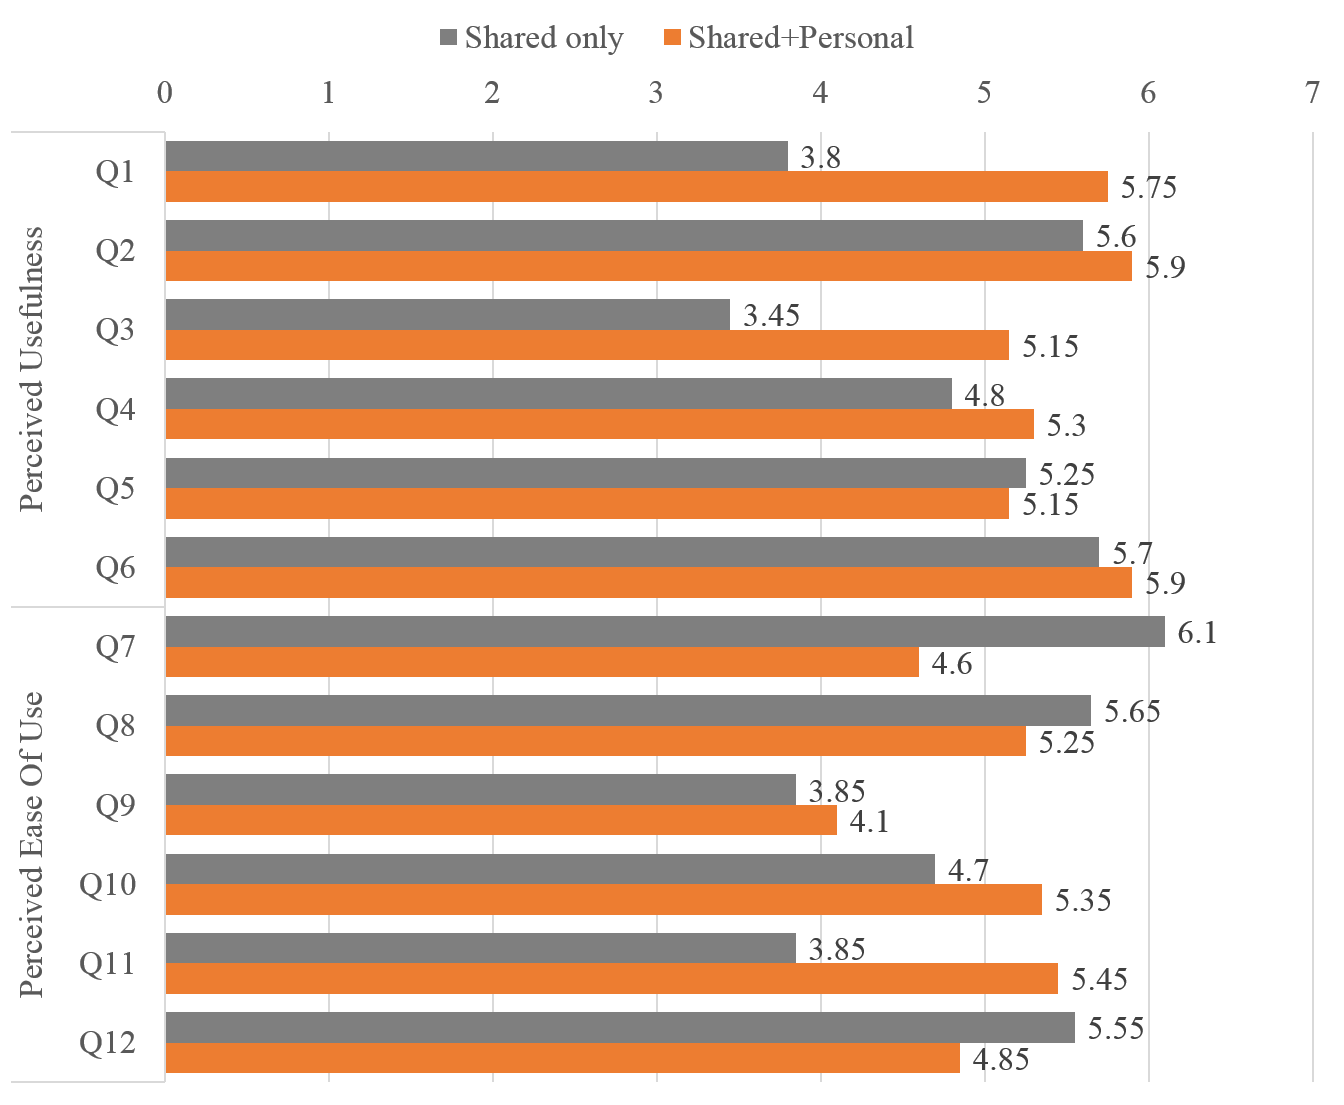
\includegraphics[width=1.0\columnwidth, height=5.5cm]{5-Experiments/pueu}
% \caption{Perceived Usefulness and Ease of Use}
% \label{fig:pueu}
% \end{figure}

% % \begin{comment}
% 그림 \ref{fig:pueu}에서 보듯이 전체적으로 평균에 비하여 높은 점수를 받았다. 특히 usefulness 항목에서는 Q2의 job performance에 관련된 내용과 Q6의 usefulness 항목이 높은 점수를 받아 제안하는 시스템이 작업의 효율을 높여줄 것이라는 의견이 많았다. 하지만, Q3의 점수가 낮게 나온 것으로 보아 생산성의 향상으로 연결되지는 않을 것으로 예상되었다. ease of use 항목에서는 Q7과 Q12가 높은 점수가 나온 것으로 보아 시스템이 쉽게 배우고 사용하기가 편리하다는 평가가 많았다. 하지만, Q9와 Q11의 점수가 낮은 것으로 보아 아직 시스템에 대한 파악이 다 되지 못하여 이해가 어려웠음을 알 수 있었다.
% 두 시스템 간의 비교를 보면, 전체적으로 combined workspace(combined using shared workspace and mobile personal workspace)에서는 usefulness 가 높게 측정된 반면, ease of use 항목은 점수가 낮았다. 특히, Q1과 Q3 항목에서 큰 차이를 보여주어, combined workspace에서 productivity가 높고 빠르게 task를 완료할 수 있을 것으로 기대되었다. 이는 construction 과정에서 발생되는 이슈에 대하여 빠르고 효율적으로 discussion 이 가능하기 때문으로 분석되었다. 반면, 모바일 시스템에 대한 학습이 필요하므로 전체적으로 Ease of Use 항목은 점수가 낮게 측정되었다.
% % \end{comment}

% % As seen in Figure \ref{fig:pueu}, overall, high scores were gained compared to the average. Especially, in the usefulness, there were lots of opinions that the proposed system would heighten work efficiency since the contents related with job performance of Q2 and the item of usefulness of Q6 gained high scores. Nonetheless, from the low score of Q3, it was predicted that it would not be linked with productivity increase. In ease of use, from seeing high scores of Q7 and Q12, there were a lot of evaluations that the system was easy to learn and convenient to use. However, from seeing low scores of Q9 and Q11, it was known that the understanding was difficult caused from insufficient grasping of the system.

% % In regards to the comparison between shared workspace only against combined workspace (combine using shared workspace and mobile personal workspace), combined workspace is perceived as higher usefulness and lower ease of use. Especially Q1 and Q3 show high differences, because the combined workspace offers efficient and rapid discussion mechanisms, so it is shown to support higher productivity and expect a fast task completion. In contrast, it has to be learnt to use on mobile applications. Overall score of Ease of Use for combined workspace showed a larger gain over a shared only workspace.


% \subsubsection{Discussion}
% % \begin{comment}
% 평가 중에 나왔던 몇 가지 코멘트 등을 통하여 시스템에 대한 주관적 평가들을 받을 수 있었다. 주로 많이 나왔던 코멘트는 현재 시스템의 하드웨어의 복잡성에 대한 의견이 많았다. 현재는 노트북에 연결하여 사용하기 때문에 시스템과 별도로 노트북이 필요하고, 연결선으로 인해 복잡하다는 반응이 많았다. 이러한 문제는 향후 Mobile Depth Camer 기술을 적용하여 Android나 iOS와 같은 모바일 버전으로 발전시켜 나가면서 해결할 수 있을 것으로 기대된다. 또한, 현재 적용된 Portable Projector에서도 화면의 FoV(Field-of-View)가 작고 밝기가 낮아서 외부 환경에서 사용하기에 적합하지 않았다. 이 또한 projector 기술의 발전과 함께 해결될 수 있을 것으로 기대된다. 마지막으로 현재 사용되고 있는 Leap Motion 기기를 이용한 손 인식 방법이 정확도는 매우 높으나, 시스템과 별도로 설치를 해야하는 문제가 있기 때문에 거추장스럽다는 의견이 많았다. 이는 시스템에 integrate 된 depth camera를 이용하여 인식함으로써 시스템을 단순화하여 제공할 수 있을 것으로 기대된다. 
% 그리고 Mobile Personal Workspace에서는 기기의 크기가 작기 때문에 세밀한 Component의 터치가 부정확하고, 선택된 Component에 대한 Visual feedback이 부족하기 때문에 작업 과정에서 오류가 자주 일어났다. 이러한 문제를 해결하기 위하여 \cite{vogel_shift:_2007}와 같은 터치 인터페이스의 개선이 적용된다면 더 높은 사용성을 제공할 수 있을 것이다.
% % \end{comment}

% % Through several comments during the evaluation, subjective evaluations of the system could be observed. Comments which came out mostly were opinions about complexity of hardware of the present system. Presently, because testing Port3DAr was used with connected laptops, there were a lot of responses that laptops are necessary apart from the system and it was complex due to connection lines. These problems can be expected to be settled from developing the system into a mobile version on smart devices using Android or iOS platforms. 
% % In addition, in the presently applied portable projector, because the Field-of-View of a screen was small and the brightness was low, it was not proper to use in external environments. It is also expected that these can be solved with the development of projector technology. Lastly, though the hand recognition method using leap motion devices presently used is high in accuracy, there were lots of opinions that it is burdensome due to the installation apart from the system. It is anticipated that the solution can be provided from the simplification of the system, by recognizing hands using a depth camera which is integrated into the system.
% % Also, for mobile personal workspaces, there are frequent errors because the device is too small to select items and there is a lack of visual feedback. To improve these problems, we implement an enhancement technique for mobile touch devices similar to \cite{vogel_shift:_2007}.
% %그리고 Mobile Personal Workspace에서는 기기의 크기가 작기 때문에 세밀한 Component의 터치가 부정확하고, 선택된 Component에 대한 Visual feedback이 부족하기 때문에 작업 과정에서 오류가 자주 일어났다. 이러한 문제를 해결하기 위하여 \cite{vogel_shift:_2007}와 같은 터치 인터페이스의 개선이 적용된다면 더 높은 사용성을 제공할 수 있을 것이다.

%\section{Conclusion}

% %!TEX root = ../construction.tex
% -*- root: ../construction.tex -*-

%-----------------------------------------------------------------------------
%	7. Conclusion and Future Work
%	목표 분량: 0.5장

\section{Conclusion and Future Work}

본 논문에서는 건축 시공 현장에서 설계 도면이나 3차원 모델과 같은 건축 정보를 실시간으로 접근하고 직관적인 인터페이스를 이용하여 이를 조작할 수 있는 포터블 2D/3D 건축 정보 인터페이스를 제안하였다. 이를 통하여 시공 현장에서 전체 모델에 대한 이해를 높일 수 있고, 특정 영역에 대한 정보를 쉽게 획득할 수 있으며, 현장에서의 수정 사항을 즉각적으로 모델에 재반영함으로써 협업의 효율을 높일 수 있었다. 특히 이를 포터블 형태의 기기에서 구현함으로써 실제 현장에서 사용이 가능하다는 장점이 있었다.

% This paper approached construction information like blueprints or 3D models in real time and proposed a portable 2D/3D construction information interface using intuitive projection design and interaction to manipulate content. Through this, understanding of all models at construction sites can be enhanced and information about special regions can be acquired easily. In addition, by re-reflecting modified matters on models promptly, efficiency of cooperation could be heightened. Particularly, by implementing them as portable, participants strongly agreed that our system could be beneficial on real construction sites.
%하지만, NUI 인식 기술 등을 향상하여 전체 시스템의 구성을 단순화하는 필요성이 있으며, HMD 등의 웨어러블 기기를 이용한 상호작용 지원 등을 통하여 실시간성과 사용성을 높일 수 있는 다른 플랫폼 과의 협업도 중요할 것으로 생각된다. 또한 Revit과 같은 상용 BIM Software와의 연동을 제공함으로써 좀 더 상세한 건축 정보 제공한다면 더욱 편리한 인터페이스로 발전할 수 있을 것으로 기대된다.
% However, there is a need to simplify overall system construction through improvements in NUI recognition technology, and cooperation with other platforms to increase usability and speed through support for interactions using wearable devices such as HMDs is important.  Development of more convenient interfaces can be expected if more detailed construction information is offered through interlocking with commercial BIM software such as Revit. 

% \begin{comment}
하지만 추가적으로 HMD 기반의 웨어러블 증강현실이나 모바일 증강현실 시스템과의 연동 기능을 제공하여 현재 작업 Context에 적합한 정보를 제공하는 연구를 진행하는 것이 필요할 것이다. 또한 Revit과 같은 상용 BIM Software와의 연동을 제공함으로써 좀 더 상세한 건축 정보 제공한다면 더욱 편리한 인터페이스로 발전할 수 있을 것으로 기대된다.

%But, for this system to work providing the interlocking functions with wearable or mobile augmented reality systems is necesary and further study is needed to process contexts in the present work. Plus, by providing interlock with common BIM software like revit, if more detailed construction information is provided, Port3DAr can be developed into a more convenient interface. 
% \end{comment}

% This paper addressed construction information such as blueprints or 3D models in real time and proposed a portable 2D/3D construction information interface using intuitive projection design and interaction to manipulate content. This can enhance understanding of models at construction sites and enables easy acquisition of information regarding specific regions. In addition, cooperation efficiency can be increased by prompt re-reflection of model modifications. In particular, participants strongly agreed that our system could be beneficial on real construction sites as a result of portable implementation. However, there is a need to simplify overall system construction through improvements in NUI recognition technology, and cooperation with other platforms to increase usability and speed through support for interaction using wearable devices such as head-mounted displays is important. Development of more convenient interfaces can be expected, if more detailed construction information is offered through interlocking with commercial BIM software such as Revit.

%%%%%%%%%%%%%%%%%%%%%%%%%%%%%%%%%%%%%%%%%%

% \subsection{This is a Subsection Heading}

% Main text paragraph.

% Main text paragraph.


% \subsubsection{This is a Subsubsection Heading}

% Main text paragraph.

% %%%%%%%%%%%%%%%%%%%%%%%%%%%%%%%%%%%%%%%%%%

% \section{Results and Discussion}

% Main text paragraph.

%% Example of a theorem:
%\begin{Theorem}
%Text text text
%\end{Theorem}

% The document text continues here.

%% Example of a proof:
%\begin{proof}[Proof of Theorem 1]
%Text text text
%\end{proof}

% The document text continues here.

% \subsection{This is a Subsection Heading}

% Main text paragraph.

% %%%%%%%%%%%%%%%%%%%%%%%%%%%%%%%%%%%%%%%%%%

% \section{Conclusions}

% Main text paragraph.


% Main text paragraph.

%%%%%%%%%%%%%%%%%%%%%%%%%%%%%%%%%%%%%%%%%%

% \acknowledgments{Acknowledgments}

% Main text.

% %%%%%%%%%%%%%%%%%%%%%%%%%%%%%%%%%%%%%%%%%%

% % \authorcontributions{Author Contributions}

% % Required if more than one author. Authorship must include and be strictly limited to researchers who have substantially contributed to the reported work. Please carefully review our criteria regarding the Qualification for Authorship: \web /instructions.

% %%%%%%%%%%%%%%%%%%%%%%%%%%%%%%%%%%%%%%%%%%

% \conflictofinterests{Conflicts of Interest}

% The authors declare no conflict of interest.

%=================================================================
% References: Variant A
%=================================================================
% Back Matter (References and Notes)
%----------------------------------------------------------
% Style and layout of the references
% \bibliographystyle{mdpi}
% \makeatletter
% \renewcommand\@biblabel[1]{#1. }
% \makeatother

% \begin{thebibliography}{999} % if there are less than 10 entries, enter a one digit number

% % Reference 1
% \bibitem{ref-journal}
% Lastname, F.; Author, T. The title of the cited article. {\em Journal Abbreviation} {\bf 2008}, {\em 10}, 142-149.

% % Reference 2
% \bibitem{ref-book}
% Lastname, F.F.; Author, T. The title of the cited contribution. In {\em The Book Title}; Editor, F., Meditor, A., Eds.; Publishing House: City, Country, 2007; pp. 32-58.

% \end{thebibliography}

%=================================================================
% References:  Variant B
%=================================================================
% Use the following option to include external BibTeX files:
\bibliography{sample}
\bibliographystyle{mdpi}

%%%%%%%%%%%%%%%%%%%%%%%%%%%%%%%%%%%%%%%%%%

%\abbreviations{Abbreviations/Nomenclature}
%
%Main text.

%%%%%%%%%%%%%%%%%%%%%%%%%%%%%%%%%%%%%%%%%%

%\appendix
%\section{Appendix Title}
%
%Main text.

\end{document}

